\documentclass[12pt,a4paper,oneside]{report}

% ========== 中文与页面设置 ==========
\usepackage[UTF8]{ctex}
\usepackage{geometry}
\geometry{a4paper, margin=2.5cm}
\usepackage{bm}
\usepackage{mathrsfs}
% ========== 数学与定理环境 ==========
\usepackage{amsmath,amssymb,amsthm,bm}
\usepackage{physics} % 物理公式快捷命令
\newtheorem{theorem}{定理}[chapter]
\newtheorem{lemma}{引理}[chapter]
\newtheorem{corollary}{推论}[chapter]
\theoremstyle{definition}
\newtheorem{definition}{定义}[chapter]
\newtheorem{example}{例题}[chapter]
\theoremstyle{remark}
\newtheorem*{remark}{注}

\setlength{\headheight}{15pt} % 将页眉高度设置为15pt
\addtolength{\topmargin}{-3pt} % 同时向上收缩页边距以补偿布局

% ========== 图表/代码/颜色支持 ==========
\usepackage{graphicx}
\graphicspath{{figure/}}
\newcommand{\insertfig}[3]{
    \begin{figure}[ht]
        \centering
        \includegraphics[width=#3\textwidth]{#1}
        \caption{#2}
        \label{fig:#1}
    \end{figure}
}
\usepackage{float}
\usepackage{caption}
\usepackage{subcaption}
\usepackage{booktabs}
\usepackage{xcolor}
\usepackage{listings}
\usepackage{esint}
\newcommand{\mb}[1]{\mathbf{#1}}
\lstset{
  language=Python,
  basicstyle=\ttfamily\small,
  keywordstyle=\color{blue},
  commentstyle=\color{gray},
  stringstyle=\color{orange},
  frame=single,
  breaklines=true
}

% ========== 目录与超链接 ==========
\usepackage{hyperref}
\hypersetup{
  colorlinks=true,
  linkcolor=blue,
  urlcolor=blue,
  citecolor=magenta
}
\usepackage{tocloft}

% ========== 页眉页脚 ==========
\usepackage{fancyhdr}
\pagestyle{fancy}
\fancyhf{}
\fancyhead[L]{电磁学笔记}
\fancyhead[R]{\leftmark}
\fancyfoot[C]{\thepage}

% ========== 章节格式美化 ==========
\usepackage{titlesec}
\titleformat{\chapter}[hang]{\Huge\bfseries}{第\thechapter 章}{1em}{}
\titleformat{\section}[hang]{\Large\bfseries}{\thesection}{0.5em}{}
\titleformat{\subsection}[hang]{\large\bfseries}{\thesubsection}{0.5em}{}

% ========== 参考文献 ==========
\usepackage[numbers]{natbib}

% ========== 封面信息 ==========
\title{\Huge\textbf{Lecture Notes on Electromagnetics}}
\author{\Large 上海交通大学 人工智能学院 \\
\Large 肖世屹}
\date{\today}

\renewcommand{\d}{\mathop{}\!\mathrm{d}}
\renewcommand{\v}{\mathop{}\!\varepsilon}
% =======================================================
\begin{document}

% --------------------- 封面 ---------------------
\maketitle
\thispagestyle{empty}
\clearpage
% --------------------- 序言 ---------------------
\chapter*{序言}
\addcontentsline{toc}{chapter}{序言} % 让“序言”出现在目录中

在本笔记中,我们系统地整理了电磁学的主要内容,
包括静电场、稳恒磁场、磁介质、电磁感和Maxwell电磁理论等五个章节。本笔记的内容基于上海交通大学大学物理(荣誉)II的课程考试要求做了适当的调整,保证学习难度和内容适于准备考试。
本笔记现已发布在Github上,读者可以访问\url{https://github.com/ShiyiXiao05/Phynotes}以获取更新。

在编写笔记的过程中,感谢我的室友陈志杰给予的排版支持,在他的帮助下这本笔记得以以美观的形式呈现给大家。同时也要感谢韩岳成、何忠颐、胡昊旻、王栎翔等同学的试读和勘误。

希望本笔记能为学习电磁学的读者提供一定帮助。
若能抛砖引玉,为读者揭开物理之美的一角,作者将不胜欣慰。

由于时间与作者水平所限,文中难免存在疏漏与错误,恳请各位读者批评指正。本人不胜感谢。
\bigskip
\begin{flushright}
肖世屹 \\
上海交通大学 人工智能学院 \\
\today
\end{flushright}
\clearpage

% --------------------- 目录 ---------------------
\tableofcontents
\clearpage

% --------------------- 正文章节 ---------------------

\chapter{静电场}
\section{库仑定律}

\begin{theorem}[库仑定律]
两个静止点电荷之间的相互作用力的大小与两个点电荷电量的乘积成正比,与他们之间的距离平方乘反比,作用力的方向沿着两点电荷间的连线,同号电荷相斥,异号电荷相吸。

设两点电荷的电量为$q_1$,$q_2$,从$q_1$指向$q_2$的径矢为$\hat{r}$,则$q_1$对$q_2$静电力为:
\[
\mathbf{F} = k_e \frac{q_1 q_2}{r^3}\mathbf{r}
\]

其中$k_e = \frac{1}{4\pi \varepsilon_0} \approx 9\times 10^9\ N\cdot m^2/C^2$,$\varepsilon_0$为真空介电常数,$\varepsilon_0 \approx 8.854\times 10^{-12}\ C^2/(N\cdot m^2)$。
\end{theorem}

\section{电场强度与高斯定律}

历史上,曾经认为带电体之间的的相互作用是直接瞬时发生的。这种作用与介质无关,也不需要传播时间,此即超距作用观点。近代物理提出了近距作用观点,也即两个点电荷之间的相互作用源于第一个点电荷在周围空间中激发出电场,然后此电场对第二个点电荷产生作用力。电场并非是形式上的手段,而是一种客观的物质。它可以携带能量,角动量,动量等以维持各种守恒定律。在静电学范围内,超距作用与近距作用是等价的。例如对于能量,我们可以认为能量由电荷携带,也可以由电场携带。

\begin{definition}[电场强度]
  我们在电场中引入以充分小的点试探电荷,以避免其对原有电场的扰动。设试探电荷为$q_0$,则试探电荷在某点受到的力$\mathbf{F}$与$q_0$的比值称为该点的电场强度,记为$\mathbf{E}$,即
  \[
  \mathbf{E} = \frac{\mathbf{F}}{q_0}
  \]
\end{definition}
\begin{theorem}[场强叠加原理]
  由于电场力是矢量,满足矢量叠加原理,那么根据定义,电场强度也满足叠加原理。即若有多个电荷$q_1,q_2,\ldots,q_n$,它们在某点产生的电场强度分别为$\mathbf{E}_1,\mathbf{E}_2,\ldots,\mathbf{E}_n$,则它们在该点产生的总电场强度为
  \[
  \mathbf{E} = \mathbf{E}_1 + \mathbf{E}_2 + \ldots + \mathbf{E}_n
  \]
\end{theorem}

我们计算点电荷产生的场强。设点电荷$q$位于原点,某点$P$的径矢为$\mathbf{r}$,则
\[
\mathbf{F} = k_e \frac{q q_0}{r^3}\mathbf{r}
\]
\[
\mathbf{E} = \frac{\mathbf{F}}{q_0} = k_e \frac{q}{r^3}\mathbf{r}
\]

原则上说,通过场强的定义,利用点电荷的场强公式和场强叠加原理可以计算任意电荷分布所产生的电场分布。而已知电场分布,任何其它带电体在电场中的运动原则上也都可以求解。因此关于电场的描述似乎已经穷尽了。然而我们并不满足于根据已知的电荷分布计算电场分布这种认识电场的途径,而是期望从不同角度揭示电场的规律性。我们知道,一定的电荷分布不仅在空间任意一点都产生一定的电场强度,形成一定的电场分布,而且空间任意一点的电场强度与邻近点的电场强度之间必然存在一定联系。寻找这种空间各点场强之间的联系可获得刻画场的规律性的最好表达,它比起直接联系场点和源点的表达更能反映场的规律性的特征。

我们先定义些概念:
\begin{definition}[电场线 \, 电通量]
  电场线是用来形象地表示电场分布的工具。它的切线方向与该点的电场强度方向相同,不同的电场线除了相交于点电荷处均不会相交。电场线总是起始于正电荷或无穷远处,而止于负电荷或无穷远处。

  元电通量被定义为:
  \[
  \d \Phi_E = E \cos\theta \d \mathbf{S} = \mathbf{E} \cdot \d\mathbf{S}
  \]
$\theta$为外法向与电场方向的夹角,$\d\mathbf{S}$为面积元矢量。

电通量就为:
  \[
  \Phi_E = \oiint_S \mathbf{E} \cdot \d\mathbf{S}
  \]

电通量表示的是穿过某个面的电场线的数量,穿过的电场线越多,电通量越大。
\end{definition}
\begin{theorem}[高斯定律]
用电通量表示高斯定理,即为:

通过一个闭合曲面\textbf{$S$}的电通量大小\textbf{$\Phi_E$}为闭合面所包含的总电荷量$\sum q$与真空介电常数$\varepsilon_0$的比值,即
  \[
  \Phi_E = \oiint_S \mathbf{E} \cdot \d\mathbf{S} = \frac{\sum q}{\varepsilon_0}
  \]

  与闭合面外的电荷无关。
\end{theorem}

证明:我们逐一来证明这个定理。首先考虑一个点电荷$q$位于闭合曲面$S$的内部,设点电荷$q$到闭合面上面积元$\d\mathbf{S}$的径矢为$\mathbf{r}$,则
  \[
  \Phi_E = \oiint_S \mathbf{E} \cdot \d\mathbf{S}= \oiint_S \frac{1}{4\pi\varepsilon_0} \frac{q}{r^2}\hat{r} \cdot (r^2 \sin\theta \d \theta \d \varphi \hat{r}) = \frac{q}{4\pi\varepsilon_0} \int_0^{\pi} \sin\theta \d \theta \int_0^{2\pi} \d \varphi
  = \frac{q}{\varepsilon_0}
  \]

对于一个位于闭合面外的点电荷,我们会发现对于一条穿过闭合面上某面元的电场线必然从另一个面元穿出,从而对电通量不产生贡献,因此其贡献的电通量为0。
由场强叠加定理,我们就可以将电荷分布视作由若干点电荷构成,从而我们得到了高斯定律。

对于一般的电荷分布,我们会将电荷分布用体电荷密度表示。于是我们可以写出高斯定律的形式:
  \[
  \oiint_S \mathbf{E} \cdot \d\mathbf{S} = \iiint_V \frac{\rho}{\varepsilon_0} \d V
  \]

散度定理告诉我们:

\[
\oiint_S \mathbf{E} \cdot \d \mathbf{S} = \iiint_V (\nabla \cdot \mathbf{E}) \d V
\]

注意到高斯面选取的任意性,我们可以得到高斯定律的微分形式:
\[
\nabla \cdot \mathbf{E} = \frac{\rho}{\varepsilon_0}
\]
% --------------------- 参考文献 ---------------------


有了高斯定理,我们就能方便地求解许多具有对称性的带电体系所产生的场强。
\begin{example}
  求解均匀带正电球壳,球体在壳外和壳内的场强分布。

  对球壳,设球壳半径为$R$,总电荷量为$Q$,注意到对称性,若场强不为零,场强的方向沿径向向外。选取球形高斯面。则球壳外的场强为:

  \[
  E \cdot 4\pi r^2 = \frac{Q}{\varepsilon_0} \Rightarrow E = \frac{1}{4\pi\varepsilon_0} \frac{Q}{r^2}
  \]

  球壳内的场强为:
  \[
  E \cdot 4\pi r^2 = 0 \Rightarrow E = 0
  \]

  对球体,设球体半径为$R$,总电荷量为$Q$。选取球形高斯面。同理球体外的场强为:
  \[
  E \cdot 4\pi r^2 = \frac{Q}{\varepsilon_0} \Rightarrow E = \frac{1}{4\pi\varepsilon_0} \frac{Q}{r^2}
  \]

  球体内的场强为:
  \[
  E \cdot 4\pi r^2 = \frac{Q}{\varepsilon_0} \cdot \frac{r^3}{R^3} \Rightarrow E = \frac{1}{4\pi\varepsilon_0} \frac{Q}{R^3} r
  \]

  方向均沿径向向外。
\end{example}

\begin{example}
  求解无限长均匀带电直线,柱面,柱体在距中心轴线$r$处的场强。

  设线电荷密度为$\lambda$,选取半径为$r$的圆柱面为高斯面。注意到这样的柱形高斯面的对称性,上下两个面的电通量为0。则
  \[
  E \cdot 2\pi r L = \frac{\lambda L}{\varepsilon_0} \Rightarrow E = \frac{\lambda}{2\pi\varepsilon_0 r}
  \]

  方向沿径向向外。

  设柱面半径为$R$,单位长柱面带电量为$\lambda$,选取半径为$r$,高为$L$的圆柱面为高斯面。则柱面外的场强为:
  \[
  E \cdot 2\pi r L = \frac{\lambda L}{\varepsilon_0} \Rightarrow E = \frac{\lambda}{2\pi\varepsilon_0 r}
  \]
  
  方向沿径向向外,柱面内场强为0。

  设柱体半径为$R$,单位长柱体带电量为$\lambda$,选取半径为$r$,高为$L$的圆柱面为高斯面。则柱体外的场强为:
  \[
  E \cdot 2\pi r L = \frac{\lambda L}{\varepsilon_0} \Rightarrow E = \frac{\lambda}{2\pi\varepsilon_0 r}
  \]
  柱体内的场强为:
  \[
  E \cdot 2\pi r L = \frac{\lambda L}{\varepsilon_0} \cdot \frac{r^2}{R^2} \Rightarrow E = \frac{\lambda}{2\pi\varepsilon_0 R^2} r
  \]
  方向均沿径向向外。
\end{example}
\insertfig{1-1.png}{柱对称高斯面示意图}{0.25}

\begin{example}
  求解无限大均匀带电平面在距平面$r$处的场强。

  考虑对无限大带电平面做镜面对称,平行于平面方向的电场强度在镜面对称下方向必然反向,但是实际上镜面对称后系统并未发生变化,于是平行平面方向上场强为0。

  设面电荷密度为$\sigma$,选取一个轴线垂直于平面的圆柱面,设其底面面积为S。则
  \[
  E \cdot 2S = \frac{\sigma S}{\varepsilon_0} \Rightarrow E = \frac{\sigma}{2\varepsilon_0}
  \]
  方向垂直于平面向外。也就是说平面产生的场强大小与距离无关,在讨论电容时这一点会经常用到。
\end{example}

电偶极子的电场我们在电势一节讨论。

\section{电势与电势的梯度}

单个点电荷产生的电场是有心力场。有心力是保守力,这一点我们已经熟知。对于一般的带电体系,我们可以将带电体划分为许多元点电荷,这样多个保守力场的叠加仍然是保守的。因此静电场是保守场。也就是说
\begin{center}
  \textbf{静电场中场强沿任意闭合环路的线积分为0.}
\end{center}

我们称之为\textbf{静电场的环路定理}。

由于静电场是保守场,我们可以引入势能的概念。对于处于静电场中的一点电荷 $q$,若其在某点 $P$ 处的电势能为 $W_P$,则可以定义电势为单位正电荷在该点所具有的电势能,即
\[
U(P)=\frac{W_P}{q}.
\]

由保守场的性质可知,电荷从点 $A$ 移动到点 $B$ 所做的功仅与初末位置有关,而与路径无关。根据功与势能的关系,有
\[
W_{AB} = W_A - W_B = q\,(U_A - U_B).
\]

因此,我们定义两点之间的电势差(potential difference)为:
\[
\Delta U = U_A - U_B = U_{AB},
\]

它表示单位正电荷从 $A$ 移动到 $B$ 时静电力所做的功。

在实际问题中,我们往往选择无穷远处或者大地的电势为0。电势满足标量叠加定律。下面我们讨论些常见带电体系的电势分布。

\begin{example}[几种典型带电体系的电势分布]

对于点电荷 \(q\)(位于原点),其电场
\[
\mathbf E(\mathbf r)=\frac{1}{4\pi\varepsilon_0}\frac{q}{r^2}\hat r.
\]
取无穷远处电势为0,则电势的表达式为
\[
V(r)=-\int_{\infty}^{r}\mathbf E(r)\cdot \d\mathbf r
=\frac{1}{4\pi\varepsilon_0}\frac{q}{r}
\]
同理,对于带电薄球壳 (半径 \(R\),总电荷 \(q\)), 其电场为:
\[
\mathbf E(r)=
\begin{cases}
\dfrac{1}{4\pi\varepsilon_0}\dfrac{q}{r^2}\hat r, & r\ge R,\\[6pt]
\mathbf 0, & r<R.
\end{cases}
\]
取无穷远处电势为0,则对球外 \(r\ge R\):
\[
V(r)=-\int_{\infty}^{r}\mathbf E(r)\cdot \d\mathbf r
=\frac{1}{4\pi\varepsilon_0}\frac{q}{r}
\]
对球内 \(r<R\),由于电场为零,电势为常数且等于表面势,即为
\[
V(r)=V(R)=\frac{1}{4\pi\varepsilon_0}\frac{q}{R}.
\]

均匀带电实心球(半径 \(R\),总电荷 \(q\)),体电荷密度 \(\rho=\dfrac{3q}{4\pi R^3}\)。,其电场为:
\[
\mathbf E(r)=
\begin{cases}
\dfrac{1}{4\pi\varepsilon_0}\dfrac{q}{r^2}\hat r, & r\ge R,\\[8pt]
\dfrac{1}{4\pi\varepsilon_0}\dfrac{q\,r}{R^3}\hat r, & r<R.
\end{cases}
\]

对球外 \(r\ge R\):
\[
V(r)=-\int_{\infty}^{r}\mathbf E(r)\cdot \d\mathbf r
=\frac{1}{4\pi\varepsilon_0}\frac{q}{r}
\]

对球内 \(r<R\),分段积分:
\[
V(r)= -\int_{\infty}^{R}\frac{1}{4\pi\varepsilon_0}\frac{q}{r'^2}\,\d r' \;-\;\int_{R}^{r}\frac{1}{4\pi\varepsilon_0}\frac{q\,r'}{R^3}\,\d r'.
\]

计算得
\[
V(r)=\frac{1}{4\pi\varepsilon_0}\frac{q}{2R}\left(3-\frac{r^2}{R^2}\right)=\frac{\rho}{6\varepsilon_0}\left(3-\frac{r^2}{R^2}\right).
\]

无限长均匀带电直线(线电荷密度 \(\lambda\))。选用以直线为轴的圆柱高斯面得径向电场
\[
E(r)=\frac{\lambda}{2\pi\varepsilon_0 r}.
\]
这里我们无法选择无穷远处势能为0,于是我们选择参考半径$r_0$处为势能零点:
\[
V(r)=-\int_{r_0}^{r}\frac{\lambda}{2\pi\varepsilon_0 r'}\,\d r'=-\frac{\lambda}{2\pi\varepsilon_0}\ln\frac{r}{r_0}.
\]

\end{example}

数学分析的知识告诉我们,之前这样定义的电势,其梯度与场强之间存在如下关系:
\[
\mathbf{E} = -\nabla U
\]

在求解带电体系的场强时,我们往往是先求解电势分布,然后求梯度得到场强。这是由于我们在直接求解场强时,面对连续带电体往往要进行矢量积分,这在数学上是相对困难的,而求解电势时只需要进行标量积分,我们对此更为熟悉。

下面我们来讨论电偶极子这一重要模型。电偶极子是指一对电量相等,符号相反,相隔距离为$l$的两点电荷系统。通常,我们认为这两点电荷之间的距离$l$相对于我们考察的点到两点电荷中心位置的距离$r$来说是充分小的。这样的条件下远离电偶极子的点所感受到的电场和电势可以用电偶极矩来描述。电偶极矩是个矢量,被定义为
\[
\mathbf{p} = q \mathbf{l}
\]

其中$\mathbf{l}$为从负电荷指向正电荷的矢量。

设两个点电荷 $+q$ 与 $-q$ 分别位于 $z$ 轴上 $\mathbf{r}_+=\frac{d}{2}\hat{\mathbf{z}}$ 与 $\mathbf{r}_-=-\frac{d}{2}\hat{\mathbf{z}}$,定义偶极距 $\mathbf{p}=q\mathbf{d}=q d\hat{\mathbf{z}}$,静电常数 $k=\dfrac{1}{4\pi\varepsilon_0}$。观测点使用球坐标表示为 $(r,\theta,\phi)$,其中 $\theta$ 是从 $+z$ 轴量起的极角。

两点电荷的电势(叠加)为
\[
V(\mathbf{r})=kq\left(\frac{1}{|\mathbf{r}-\frac{d}{2}\hat{\mathbf{z}}|}
-\frac{1}{|\mathbf{r}+\frac{d}{2}\hat{\mathbf{z}}|}\right).
\]

令 $\mathbf{a}=\pm\frac{d}{2}\hat{\mathbf{z}}$,并利用远场展开(当 $r\gg d$ 时,对小量 $\mathbf{a}$ 作泰勒展开)
\[
\frac{1}{|\mathbf{r}-\mathbf{a}|}
=\frac{1}{r}\frac{1}{\sqrt{1-2\frac{\hat{\mathbf{r}}\cdot\mathbf{a}}{r}+\frac{a^2}{r^2}}}
\approx \frac{1}{r}\left(1+\frac{\hat{\mathbf{r}}\cdot\mathbf{a}}{r}+\mathcal{O}\!\left(\frac{a^2}{r^2}\right)\right).
\]

代入得(仅保留关于 $d$ 的一阶项)
\[
\begin{aligned}
V(\mathbf{r})
&\approx kq\left(\frac{1}{r}+\frac{\hat{\mathbf{r}}\cdot(\tfrac{d}{2}\hat{\mathbf{z}})}{r^2}
-\frac{1}{r}-\frac{\hat{\mathbf{r}}\cdot(-\tfrac{d}{2}\hat{\mathbf{z}})}{r^2}\right) \\
&= kq\frac{d\,(\hat{\mathbf{r}}\cdot\hat{\mathbf{z}})}{r^2}
= k\frac{\mathbf{p}\cdot\hat{\mathbf{r}}}{r^2}.
\end{aligned}
\]
由于 $\hat{\mathbf{r}}\cdot\hat{\mathbf{z}}=\cos\theta$,得电偶极子的电势表达式
\[
\,V(r,\theta)=k\frac{p\cos\theta}{r^{2}}\,
\]

极坐标坐标中标量函数 $V(r,\theta)$ 的梯度为(与 $\phi$ 无关时)
\[
\nabla V = \frac{\partial V}{\partial r}\,\hat{\mathbf{r}}
+ \frac{1}{r}\frac{\partial V}{\partial \theta}\,\hat{\boldsymbol{\theta}}.
\]
对 $V(r,\theta)=k p\cos\theta\,r^{-2}$ 求偏导:
\[
\frac{\partial V}{\partial r}
= k p\cos\theta\cdot(-2)r^{-3} = -\frac{2k p\cos\theta}{r^{3}},
\]
\[
\frac{\partial V}{\partial \theta}
= k p\cdot(-\sin\theta)\,r^{-2} = -\frac{k p\sin\theta}{r^{2}}.
\]
因此
\[
\nabla V = -\frac{2k p\cos\theta}{r^{3}}\,\hat{\mathbf{r}}
- \frac{1}{r}\frac{k p\sin\theta}{r^{2}}\,\hat{\boldsymbol{\theta}}
= -\frac{2k p\cos\theta}{r^{3}}\,\hat{\mathbf{r}}
- \frac{k p\sin\theta}{r^{3}}\,\hat{\boldsymbol{\theta}}.
\]
由 $\mathbf{E}=-\nabla V$ 得
\[
\mathbf{E}(r,\theta)=\frac{2k p\cos\theta}{r^{3}}\,\hat{\mathbf{r}}
+ \frac{k p\sin\theta}{r^{3}}\,\hat{\boldsymbol{\theta}},
\]

\section{静电场中的导体和电容}
电荷不能离开具有静止质量的粒子而独立存在,所以电荷的移动必定伴随着带电粒子的运动,能够自由移动的带电粒子称为\textbf{载流子},附着在载流子上的电荷称为\textbf{自由电荷}。导体的特点是其内部存在大量载流子及其携带的自由电荷,这些自由电荷在电场中受力产生移动,使电荷分布发生改变,而电荷分布的变化又会反过来影响电场的分布,直到导体内部电场处处为0,自由电荷不再移动。

因此,我们把导体上电荷分布以及导体内外电场分布不再变化的状态称为\textbf{静电平衡。在静电平衡状态下,导体内部电场处处为0。}这是因为若有电场不为0的点,其自由电荷必然发生移动。

下面作些说明。引人导体后,由于电荷和电场的分布相互影响、相互制约,它们最后达到的平衡分布都是不能预先判知的。我们处理问题的办法不是去分析电场、电荷在相互作用下怎样达到平衡分布的复杂过程,而是假定这种平衡分布已经达到,以上述平衡条件为出发点,结合静电场的普遍规律(如高斯定理,环路定理等)去进一步分析问题。

由静电平衡的这一定义,我们自然地得出以下结论:
\begin{itemize}
  \item 导体内部电场处处为0。
  \item 导体是等势体,导体表面是等势面。
  
  由于导体内部电场为0,导体上任意两点间电势差为0。
  \item 导体内部没有自由电荷,所有自由电荷均分布在导体表面。
  
  用高斯定理容易证明这一点。在导体内任意取一闭合面。由于面上的点都在导体内,场强为0。所以闭合面上电通量为0。由高斯定理,闭合面内电荷总量为0。由于闭合面的任意性,导体内电荷密度处处为0。因此如果导体带电,所有电荷均分布在导体表面。

  \item 导体表面电场与表面法线方向一致,且大小与表面电荷密度$\sigma$成正比,即
  \[
  E = \frac{\sigma}{\varepsilon_0}
  \]
  我们取一个柱形高斯面,其底面面积为$\d S$,其侧棱方向与场强方向平行。这样侧面上电通量为0。上底面在导体外,下底面在导体内,导体内部电通量为0,于是有:
  \[
  E \d S = \frac{\sigma \d S}{\varepsilon_0}
  \Rightarrow E = \frac{\sigma}{\varepsilon_0}
  \]

  \item 带空腔的导体,若腔内无自由电荷,则空腔内壁无电荷。若腔内有自由电荷$q$,则其内壁带电,且总带电量为$-q$。
  
  我们也用高斯定理证明。我们在此空腔导体内取一个包含空腔和空腔内壁的闭合面。容易知道其总电通量为0。若腔内无自由电荷,则腔内壁净电荷为0。若腔内壁上一些区域带正电,一些带负电,则正电荷发出的电场线既不能伸向无穷远(导体内无电场线),也不能伸向导体上的负电荷(导体是等势体),则腔内只能无电荷。

  \item 带空腔导体若不接地,腔内电场不受导体外电场的影响,导体外电场可以受腔内电场的影响。若带空腔导体接地,则腔内电场和导体外电场相互不受影响。
  
  总结来看,对于静电平衡下带空腔导体,其外部带电体不会影响空腔内部的电场分布,当导体接地时,其空腔内部的带电体不会对导体外的电场分布有影响,这效应被称为\textbf{静电屏蔽}。
\end{itemize}

静电场问题往往是,给定各导体的形状,相对位置,各导体的电量或电势来确定空间的电场分布。静电场唯一性定理告诉我们,给定静电场空间各导体的几何形状,空间内自由电荷的分布和导体上的总电量或者电势,那么我们可以\textbf{唯一}确定空间中各点的电场强度,这被我们称之为静电场唯一性定理。也就是说,给定自由电荷和边界条件,我们会得到唯一确定的电场分布,这保证了如果我们能够通过某些方式直接猜测得到电荷的最终分布,只要其满足边界条件,这就是唯一正确的解。

对于孤立导体,电荷在其导体表面上的分布与其表面的曲率半径成反比。当导体的形状和大小确定时,根据电势的叠加原理,孤立导体所带电量应该与其电势成正比,于是我们定义孤立导体所带电量与其电势的比值为孤立导体的电容$C$:
\[
C=\frac{q}{V}
\]
例如对于球形的孤立导体,$V=\frac{q}{4\pi\varepsilon_0R}$,$C=4\pi\varepsilon_0R$.

当导体附近有其他的导体或带电体时,其电势会受到其他导体或带电体的影响。于是为了消除这种影响,我们利用静电屏蔽,将互不相连的两个导体构成闭合或近似闭合的空腔导体,从而使得两导体电势差的正比关系与其他的带电体无关。这样的导体系统被称为\textbf{电容器}。则电容器的电容为:
\[
C=\frac{q}{V_A-V_B}
\]

\begin{example}
求解平行板电容器,圆柱形电容器,球形电容器的表达式。设介质的介电常数为$\varepsilon$.

设平行板电容器的面积为 $A$,板间距为 $d$,忽略边缘效应。
  取面电荷密度为 $\sigma$,由高斯定律,板间电场大小为
  \[
    E=\frac{\sigma}{\varepsilon}.
  \]
  电势差
  \[
    V=\int_0^d E\,\mathrm{d}x=E d=\frac{\sigma d}{\varepsilon}.
  \]
  由于总电荷 $Q=\sigma A$,由 $C=Q/V$ 得
  \[
    C=\frac{Q}{V}=\frac{\sigma A}{\sigma d/\varepsilon}=\frac{\varepsilon A}{d}.
  \]

  设同轴圆柱电容器内导体半径为 $a$,外导体内半径为 $b$,长度为 $L$,假设 $L\gg b$。设线电荷密度为 $\lambda=Q/L$。板间距轴心距离为r处电场强度为,
  \[
    E(r)=\frac{\lambda}{2\pi\varepsilon r}.
  \]
  两导体间电势差
  \[
    V=\int_a^b E(r)\,\mathrm{d}r=\frac{\lambda}{2\pi\varepsilon}\int_a^b\frac{1}{r}\,\mathrm{d}r
    =\frac{\lambda}{2\pi\varepsilon}\ln\frac{b}{a}.
  \]
  因此电容
  \[
    C=\frac{Q}{V}=\frac{\lambda L}{(\lambda/2\pi\varepsilon)\ln(b/a)}=\frac{2\pi\varepsilon L}{\ln(b/a)}.
  \]
  每单位长度电容为
  \[
    C'=\frac{C}{L}=\frac{2\pi\varepsilon}{\ln(b/a)}.
  \]

  设两个同心导体球,内半径为 $a$,外半径为 $b$
  
  对半径 $r$($a<r<b$)的高斯球面,电场为
  \[
    E(r)=\frac{Q}{4\pi\varepsilon r^2}.
  \]
  电势差
  \[
    V=\int_a^b E(r)\,\mathrm{d}r=\frac{Q}{4\pi\varepsilon}\int_a^b\frac{1}{r^2}\,\mathrm{d}r
    =\frac{Q}{4\pi\varepsilon}\Big(\frac{1}{a}-\frac{1}{b}\Big).
  \]
  因此电容为
  \[
    C=\frac{Q}{V}=\frac{4\pi\varepsilon}{\dfrac{1}{a}-\dfrac{1}{b}}=\frac{4\pi\varepsilon ab}{\,b-a\,}.
  \]
  当外球半径 $b\to\infty$(孤立带电球)时,
  \[
    C=4\pi\varepsilon a.
  \]
\end{example}

\begin{example}
推导电容器的并联与串联等效电容公式。

设有 $n$ 个电容器 $C_1, C_2, \dots, C_n$ 并联,电压相同为 $V$。

每个电容器上的电荷为:
\[
Q_i = C_i V,\qquad i=1,2,\dots,n.
\]

总电荷为:
\[
Q_{\text{总}} = \sum_{i=1}^n Q_i = \sum_{i=1}^n C_i V.
\]

等效电容 $C_{\text{eq}}$ 定义为:
\[
Q_{\text{总}} = C_{\text{eq}} V,
\]

因此得到并联公式:
\[
C_{\text{eq}} = \sum_{i=1}^n C_i.
\]

设有 $n$ 个电容器 $C_1, C_2, \dots, C_n$ 串联,电荷相同为 $Q$。

每个电容器上的电压为:
\[
V_i = \frac{Q}{C_i},\qquad i=1,2,\dots,n.
\]

总电压为:
\[
V_{\text{总}} = \sum_{i=1}^n V_i = \sum_{i=1}^n \frac{Q}{C_i}
= Q \sum_{i=1}^n \frac{1}{C_i}.
\]

等效电容 $C_{\text{eq}}$ 定义为:
\[
Q = C_{\text{eq}} V_{\text{总}},
\]

代入上式得到:
\[
Q = C_{\text{eq}}\, Q \sum_{i=1}^n \frac{1}{C_i}.
\]

两边约去 $Q$($Q\neq 0$),得串联公式:
\[
\frac{1}{C_{\text{eq}}} = \sum_{i=1}^n \frac{1}{C_i}.
\]
\end{example}

\section{静电能}
移动一个体系中的电荷,就需要抵抗静电力所做的一些功,这些功指的是静电能的变化。想要确定一个体系的总静电能有多少,需要说明是相对什么状态。我们通常规定,设想将体系中的所有电荷分离到彼此相距无穷远的地方,规定此状态下静电能为0。

设带电体系由若干个带电体组成,则静电能由各带电体之间的相互作用能之和$W_e$以及各带电体的自能$W_{\text{自}}$之和组成。我们先考虑点电荷体系且只考虑相互作用能。

只有两个点电荷时,设两点电荷分别为$q_1$和$q_2$,它们之间的距离为$r_{12}$,则
\[
W_{12}= W_{21} = k_e \frac{q_1 q_2}{r_{12}}
\]
把储能改写为$W_e=\frac{1}{2}(W_{12}+W_{21})$。显然我们可以将其推广到N点电荷体系,得到:
\[
W_e = \frac{1}{2} \sum_{i=1}^N \sum_{\substack{j=1 \\ j\neq i}}^N k_e \frac{q_i q_j}{r_{ij}} = \frac{1}{2} \sum_{i=1}^N q_i U_i
\]

对于连续分布的电荷,我们可以给出积分形式的静电能:
\[
W_e = \frac{1}{2} \iiint_V \rho U \d V \; \text{or} \; W_e = \frac{1}{2} \iiint_V \sigma U \d S    
\]

\begin{example}
证明电偶极子在外电场中的势能公式 \(U=-\mathbf{p}\cdot\mathbf{E}\)。

设偶极子由两点电荷 \(\pm q\) 组成,间距为 \(\mathbf{d}\),则偶极矩为
\(\mathbf{p}=q\mathbf{d}\)。

正负电荷在外电场 \(\mathbf{E}\) 中的电势能分别为
\[
U_{+}=q\varphi(\mathbf{r}+\tfrac{\mathbf{d}}{2}),\qquad
U_{-}=-q\varphi(\mathbf{r}-\tfrac{\mathbf{d}}{2}).
\]

将外势 \(\varphi\) 在 \(\mathbf{r}\) 处作泰勒展开到一阶:
\[
\varphi(\mathbf{r}\pm\tfrac{\mathbf{d}}{2})
\simeq \varphi(\mathbf{r})\pm \frac{\mathbf{d}}{2}\cdot\nabla\varphi(\mathbf{r}).
\]

故总能量为
\[
U=U_{+}+U_{-}
= q\left[\varphi(\mathbf{r})+\frac{\mathbf{d}}{2}\cdot\nabla\varphi\right]
-q\left[\varphi(\mathbf{r})-\frac{\mathbf{d}}{2}\cdot\nabla\varphi\right]
= q\mathbf{d}\cdot\nabla\varphi(\mathbf{r}).
\]

而 \(\mathbf{E}=-\nabla\varphi\),所以
\[
\boxed{U=-\mathbf{p}\cdot\mathbf{E}(\mathbf{r})}.
\]
\end{example}


\begin{example}
计算薄带电球壳与均匀带电实心球的静电自能。

球壳面电荷密度为
\[
\sigma=\frac{Q}{4\pi R^2}.
\]
球面上任一点的电势(由整个球壳产生)为
\[
U=\;k\frac{Q}{R}\quad(\text{在球面上势为常数}).
\]
代入面积分公式得
\[
\begin{aligned}
W_{\mathrm{shell}}=\tfrac{1}{2}\iint_{S}\sigma\,U\,\mathrm{d}S
= \frac{Q^2}{8\pi\varepsilon_0 R}.
\end{aligned}
\]
\end{example}

球体的体电荷密度为
\[
\rho=\frac{Q}{\tfrac{4}{3}\pi R^3}=\frac{3Q}{4\pi R^3}.
\]
球内任一点 \(r\le R\) 处由已知电荷产生的电势(相对于无穷远)为(已知结果)
\[
U(r)=k\frac{Q}{2R}\Big(3-\frac{r^2}{R^2}\Big).
\]
于是体积分为
\[
\begin{aligned}
W_{\mathrm{sphere}}
&=\tfrac{1}{2}\int_{V}\rho\,U(r)\,\mathrm{d}V
=\tfrac{1}{2}\int_{0}^{R}\rho\,U(r)\,4\pi r^2\,\mathrm{d}r \\
&=\tfrac{1}{2}\int_{0}^{R}\frac{3Q}{4\pi R^3}\cdot
\left(k\frac{Q}{2R}\Big(3-\frac{r^2}{R^2}\Big)\right)\,4\pi r^2\,\mathrm{d}r \\
&= \frac{3Q^2}{16\pi\varepsilon_0R^4}
\int_{0}^{R}\big(3r^2-\frac{r^4}{R^2}\big)\,\mathrm{d}r. \\
&= \frac{3Q^2}{20\pi\varepsilon_0 R}.
\end{aligned}
\]

假如电子被当作点电荷,将会出现静电能的发散困难。如果我们处理为带电球,我们假设这些静电能与电子的静止能量$m_ec^2$相等,我们得到电子的经典半径:
\[
r_e=\frac{e^2}{4\pi\varepsilon_0m_ec^2}\approx 2.8\times10^{-15}m
\]
 
虽然这一长度决不代表电子的线度,但是这一半径在电子散射等方面仍然可以作为电子的一个特征长度相关。

先前我们提到的这些静电能公式都是与电荷相联系的,这似乎给我们印象说静电能储存在电荷上。但是我们在一开始即表明这一观点实际上是不完全正确的,我们下面介绍如何用电场储能计算静电能。

对于真空,单位体积内存有的静电能称为电场的能量密度。电场的能量密度为:
\[
w_e=\frac{1}{2}\varepsilon_0E^2
\]

对于均匀各向同性电介质中,静电场能量密度为
\[
w_e=\frac{1}{2}\varepsilon_r\varepsilon_0E^2
\]

于是计算真空中非匀强电场的电场能时:
\[
W_e = \frac{1}{2} \iiint_V \varepsilon_0 E^2 \d V
\]

对于电容器,我们有储能公式:
\[
Q=\frac{1}{2}CU^2 = \frac{Q^2}{2C} = \frac{1}{2}QU
\]

\section{电介质}
电介质就是绝缘介质,它们是不导电的。从微观的角度看,电介质分子中的电子和原子核结合的很紧密,电子处于束缚状态,其中几乎没有自由电荷。但电介质分子在外电场的作用下仍然会产生相应的电场,为了描述这种变化,我们将电介质分子的正电荷和负电荷都集中到一个点上,这样每一个分子就形成了一个电偶极子,大量这样的电偶极子叠加就可以产生相应的电场。

历史上,人们对电介质的研究源于其对电容的影响。在平行板电容器中加入导体板,其电容会显著增大,这是由于导体表面由于外电场的存在出现了感应电荷,感应电荷产生的电场导致新插入的导体板间不存在电场,导致两板间的电势差减少。而电介质也具有类似的功能。插入电介质后,电容器的电容也有增加。我们用相对介电常数$\varepsilon_r$来表征电介质的这种增大电容的本领。

如果一个点电荷$q$的周围放满相对介电常数为$\varepsilon_r$的电介质,其电场强度的表达式将修改为:
\[
\mathbf{E}=\frac{q}{4\pi\varepsilon_r\varepsilon_0r^2}\hat{r}
\]

通常我们将分子按照其电荷分布特征分为极性分子和非极性分子,极性分子指正负电荷中心不重合的分子,非极性分子恰好相反。极性分子本身就具有一定的电偶极矩,在外场的作用下,这种偶极矩会进一步增大。

对于非极性分子,我们考虑一个简单模型,假定该分子位于一个匀强电场中。其中的原子核将会沿着电场方向移动,电子将沿着电场的反方向移动,直到这两者间的引力再次达到平衡,这样就产生了一个与外场方向相同的电偶极矩。像这样,非极性分子在外场的作用下,其正负电荷中心将会分离,产生电偶极矩,体现出与极性分子相似的特性,这种现象叫做极性分子的极化。

无外场作用时,热运动导致每个分子的电偶极矩方向是随机的,统计上电偶极矩相互抵消,不产生电场。在外场作用下,极性分子和非极性分子都会产生总计不为0的电偶极矩,由此产生附加的电场,这种电场被称为极化电场。总电场即为外电场与极化电场的和。

在前面的讨论中,我们发现在电介质中任一宏观小微观大的体积元内的电偶极矩矢量和不为零。于是我们引入极化强度$\mathbf{P}$,定义为介质单位体积内分子电偶极矩的矢量和,即:
\[
\mathbf{P}=\frac{\sum_i \mathbf{p_i}}{\Delta V}
\]

实验上表明,对于\textbf{均匀各向同性线性}电介质,在外加电场后,其极化强度为
\[
\mathbf{P}=\chi_e \varepsilon_0 \mathbf{E}
\]
这里$\chi_e$被称为极化率,而必须要加以注意的是,这里的$\mathbf{E}$指的是总电场而非一开始加入的外场。

以块状电介质为例,虽然在足够小的区域内正电荷负电荷足够靠近,可以认为局部区域内是电中性的,但是在电介质的表面会产生相应的电荷积累,这种电荷被称为\textbf{极化电荷}。这样的极化电荷会产生相应的电场$\mathbf{E'}$,这种电场被称为\textbf{退极化电场}。这是因为极化电荷的电场与外加电场方向相反,会导致外场的削弱,从而减弱极化,因而称退极化电场。也就是说总电场为
\[
\mathbf{E}=\mathbf{E_0}+\mathbf{E'}
\]

下面推导电介质表面处极化电荷面密度与极化强度之间的关系。

取一个斜柱体,其一个底面位于电介质内部,另一个位于电介质表面。其轴线与极化强度$\mathbf{P}$平行。这样我们可以写出其内部的电偶极矩矢量和大小为:
\[
|\sum_i\mathbf{p_i}|=P\Delta V = \mathbf{P} \cdot \hat{e_n} \Delta S \Delta x
\]
而注意到整个柱体被视为电偶极子时,其电偶极矩的大小又被写为:
\[
|\sum_i\mathbf{p_i}| = \sigma' \Delta S \Delta x
\]
消掉小量,我们得到\textbf{极化电荷面密度与极化强度的关系}:
\[
\sigma' = \mathbf{P} \cdot \hat{e_n} = P\cos\theta
\]

根据这一推导,假设某平行板电容器充满电介质。设板上原有的自由电荷的面密度为$\sigma_0$。设极化电荷面密度为$\sigma'$。于是电介质中的场强为 
\[
E=\frac{\sigma_0-\sigma'}{\varepsilon_0}
\]

极化强度为:
\[
P=\chi_e\varepsilon_0 E=\chi_e(\sigma_0-\sigma')
\]

又根据我们前面的公式:
\[
P=\sigma'
\]

这样我们解得
\[
\sigma' = \frac{\chi_e}{1+\chi_e}\sigma_0 \, E= \frac{1}{1+\chi_e} \frac{\sigma_0}{\varepsilon_0}
\]

于是填充电介质后的电容增大为:
\[
C=(1+\chi_e)C_0 \Rightarrow \varepsilon_r = 1+\chi_e
\]

下面我们考虑有电介质时的高斯定理。我们取一个任意的闭合面,我们知道其表面极化电荷的总量为$\oiint_S \mathbf{P} \cdot \d \mathbf{S}$, 注意到极化电荷的总量为0。于是我们得到其包围的极化电荷总量为$-\sum q'$。于是我们得到这样的极化高斯定理:
\[
\oiint_S \mathbf{P} \cdot \d \mathbf{S}  = -\sum_V q'
\]
我们再写出相应的高斯定理:
\[
\oiint_S \varepsilon_0 \mathbf{E} \cdot \d \mathbf{S}  = \sum_V q
\]

两个式子相加,我们定义新的\textbf{电位移矢量}$\mathbf{D}$,
\[
\mathbf{D} = \varepsilon_0\mathbf{E}+\mathbf{P}
\]

利用自由电荷与总电荷的关系$q = q_f + q' $, 我们得到了
\[
\oiint_S \mathbf{D} \cdot \d \mathbf{S}  = \sum_V q_f
\]
这式子被称为有电介质时的高斯定理,这表明了我们可以由自由电荷直接处理一些事情,而不必直接计算相对复杂的极化过程。对于各向同性线性电介质,有
\[
\mathbf{D} = \varepsilon_0 \mathbf{E}+\mathbf{P} = \varepsilon_0 (1+\chi_e)\mathbf{E} = \varepsilon_0\varepsilon_r\mathbf{E}=\varepsilon \mathbf{E}
\]
我们通过一道例题来讲解这一问题:
\begin{example}
  一个半径为$R$的带电量为$Q$的导体球,在其外同心地包裹一层各向同性均匀电介质球壳,其内外半径为$a,b$,相对介电常量为$\varepsilon_r$,计算球壳内各点的极化强度大小和表面上的极化电荷面密度。

  我们取球形高斯面,则容易得到:
  \[
  D\cdot4\pi r^2 = Q \Rightarrow D=\frac{Q}{4\pi r^2}
  \]

  由$\mathbf{D} = \varepsilon_0\varepsilon_r\mathbf{E}$,得到
  \[
  E=\frac{D}{\varepsilon_0\varepsilon_r}=\frac{Q}{4\pi \varepsilon_0\varepsilon_r r^2}
  \]

  由$vec{P}=\chi_e \varepsilon_0 E = \varepsilon_0(\varepsilon_r-1)\mathbf{E}$,得到
  \[
  P=\frac{(\varepsilon_r-1)Q}{4\pi \varepsilon_rr^2}
  \]
  则内外表面极化电荷面密度为:
  \[
  \sigma'_a=-P_a = \frac{(1-\varepsilon_r)Q}{4\pi \varepsilon_ra^2},\sigma'_b=P_b = \frac{(\varepsilon_r-1)Q}{4\pi \varepsilon_rb^2},
  \]
\end{example}
\section{第一章补充例题}
导体与电介质这个部分是不那么好理解的,我们这里给出几道题目,供读者参考。
\begin{example}
真空中有一场强为$E_0$的均匀场,在此电场中放入一相对介电常数为$\varepsilon_r$的
均匀极化介质球,求这介质球内任意一点的场强。

这是一道很经典的极化球的问题。我们在求解这道题目问题之前,我们要先对如何处理这种题目做一个说明。我们先前曾经说过,极化电荷的作用效果是削弱原有电场的作用,因而被称为退极化场。而不同的电荷分布会产生不同的退极化场,因而我们这里得到的退极化场大小与极化强度矢量的关系并\textbf{不是}普适的!

球体内的总场是外加电场$E_0$与退极化场$E'$的叠加。我们先假设球体内的场强为$E$.当介质球均匀极化时,其极化电荷分布是均匀的。介质球的极化可以被视作两个体电荷密度为$\pm\rho$的球分开了极小的距离$\mathbf{l}$.我们可以证明,这样的极化电荷分布在球体内部产生的场强为:
\[
E'=-\frac{\rho}{3\varepsilon_0}\mathbf{l}
\]
极化电荷体密度来源于电偶极子的叠加,根据我们对极化强度的定义,我们可以得到:
\[
\mathbf{P}=\frac{\sum_i \mathbf{p_i}}{\Delta V}=\frac{\Delta q \mathbf{l}}{\Delta V}=\frac{\rho \Delta V \mathbf{l}}{\Delta V}=\rho \mathbf{l}
\]
于是代入上式,我们得到极化球内退极化场与极化强度的关系:
\[
E'=-\frac{\mathbf{P}}{3\varepsilon_0}
\]
我们还有介质方程:
\[
\mathbf{P}= \chi_e \varepsilon_0 \mathbf{E}= (\varepsilon_r-1)\varepsilon_0 \mathbf{E}
\]
总场与退极化场的关系:
\[
E=E_0+E
\]
以上诸式联立,我们解得:
\[
E=\frac{3}{\varepsilon_r+2}E_0
\]
\end{example}

下面我们介绍分区均匀线性各向同性介质问题的解法。我们需要分两种情况讨论。

\textbf{(1)介质分界面与电场线重合.
(2)介质分界面与等势面重合.
}

先来看第一种\textbf{介质分界面与电场线重合}。该种情况下,我们这样理解。假定我们首先存在着已经给定的自由电荷分布,在达到平衡之后,我们以电场线为界填入不同介电常数的均匀各向同性介质,我们需要思考的是,这样的介质填充会影响电场线的位型分布吗?我们的答案是不会。首先注意到电场强度是沿着介质界面的。$P$在界面上是没有法向分量的,因此两种介质在分界面上面的极化电荷为0.因而极化电荷只能出现在介质和导体的边界上。因为我们可以假定在填充入介质前后,会由自由电荷的变化来补偿极化电荷的分布,使得形式上保持电荷分布的不变。这里我们找到的是一个解,由静电场唯一性定理我们得到这是唯一的解。当然这样的补偿可能导致电荷总量的变化,于是空间电场的分布只差一个常数因子$\alpha$.这样,我们讨论的电场分布可以表示为:
\[
E = \alpha E_0
\]
其中$E_0$是没有介质时的电场分布。如果我们希望确定$\alpha$,我们可以使用介质中的高斯定理对各介质积分得到等式。

我们最常见的简单情况是对称的一维问题,也就是只与一个空间坐标有关。这样,我们的不必引入$\alpha$.因为$E_0$是具有对称性,于是我们也可以直接通过积分来确定$E$. 具体地说:
\[
\oiint_S \mathbf{D} \cdot \d \mathbf{S}  = \sum_i \sum_{S_i}\v_i \v_0 E \cdot \d S = \v_0 E \sum_i \v_i S_i
= Q_0
\]
由上式计算出$E$.下面看例题。

\begin{example}
球形电容器带电量为$Q_0$,极板间充满了$\v_1$,$\v_2$两种介质,求$D,E$.
\insertfig{1-2.png}{例题1-11题图}{0.25}

利用高斯定理:
\[
\oiint_S \mathbf{D} \cdot \d \mathbf{S}  = 2\pi r^2 (D_1+D_2) =2\pi r^2 E(\v_1+\v_2) = Q_0
\]

解得:
\[
E=\frac{Q_0}{2\pi r^2(\v_1+\v_2)}, \text{方向沿着径向向外}
\]
\[
D_1 = \v_1 E = \frac{\v_1 Q_0}{2\pi r^2(\v_1+\v_2)}, D_2 = \v_2 E = \frac{\v_2 Q_0}{2\pi r^2(\v_1+\v_2)}
\]

\end{example}
再来看一题.
\begin{example}
  平行板电容器,带电$Q-0$,板间距$d$,长度$a$,宽度$b=b1+b2$。介电常数为$v_1$和$v_2$。求$C$和极板上自由电荷$\sigma_e$.

  \insertfig{1-3.png}{例题1-12题图}{0.25}

  同样地,由高斯定理:
  \[
  \oiint_S \mathbf{D} \cdot \d \mathbf{S}  = E(b_1\v_1+b_2\v_2) = Q_0
  \Rightarrow E=\frac{Q_0}{(b_1\v_1+b_2\v_2)} , C  = \frac{Q_0}{Ed} = \frac{b_1\v_1+b_2\v_2}{d}, 
  \]

  \[
\sigma_{e1} = D_1 = \v_1 E = \frac{\v_1 Q_0}{(b_1\v_1+b_2\v_2)}, \sigma_{e2} = D_2 = \v_2 E = \frac{\v_2 Q_0}{(b_1\v_1+b_2\v_2)}
  \]

我们看到自由电荷在极板上分布是不均匀的,但是这种不均匀性恰好是被极化电荷补偿而导致总电荷密度是均匀分布的。电容器内电场仍然是均匀分布的。

上面的结果自然可以用电容器并联得到结果,但是这样的做法显然是更加基本的。
\end{example}

再来看第二种\textbf{介质分界面与等势面重合}. 这种情况下我们可以直接给出结论:
\[
D = \v_0 E_0
\]
$E_0$是自由电荷产生的静电场。注意!无论是在真空中还是在介质中,电荷产生场的方式是不会变化的!当我们说介质的影响时,其实是在讨论极化电荷对原场的削弱作用!而自由电荷产生的原场是不会变化的!只是总场因为退极化场的存在而发生了变化。

我们只需证明$D$和$\v_0 E_0$满足相同的高斯定理和环路定理即可.
\[
\oiint_S \mathbf{E} \cdot \d \mathbf{S}  = \frac{Q_0}{\v_0},
\oiint_S \mathbf{D} \cdot \d \mathbf{S}  = Q_0
\]
于是这两个矢量满足相同的高斯定理.

$\v_0 E_0$满足环路定理显然是可以由$E_0$满足环路定理给出:
\[
\oint_L \mathbf{E_0} \cdot \d \mathbf{l}  = 0 
\]
一般而言,$D$是不满足环路定理的,但是对这种特殊情况我们可以证明其满足环路定理.
  \insertfig{1-4.png}{证明环路定理}{0.25}

我们任取一个闭合回路,则:
\[
\oint_L D \cdot \d \mathbf{l} = \sum_i^N \int_{L_i} D_i = \sum_i^N \v_i \int_{L_i} E_i
\]
然而注意到各介质界面均为等势面,于是我们有:
\[
\int_{l_1} E \cdot \d l =U_{AB} =0, \int_{l_N} E \cdot \d l =U_{DC} =0 
\]

\[
\int_{l_{i1}} E_i \cdot \d l+\int{l_{i2}} E_i \cdot \d l = U_{GE}+U{FH}=U_F - U_H+U_G-U_E = 0
\]
于是我们证明了:
\[
\oint_L \mathbf{D} \cdot \d \mathbf{l}  = 0
\]
至此我们证明了$D$和$\v_0 E_0$满足同样的高斯定理和环路定理,静电场的唯一性定理告诉我们这是唯一的解。

这类问题的处理步骤是:
\begin{itemize}
  \item 去掉介质,计算系统给定的自由电荷分布带来的场强$E_0$,由$D=\v_0 E_0$得到$E$.
  \item 分区域利用$E_i=\frac{\v_0 E_0}{\v_i}$计算各介质内的电场强度.
\end{itemize}

下面来看例题.
\begin{example}
  平行板电容器,两板间充满厚度分别为$d_1$,$d_2$,介电常数为$v_1$,$V_2$的两层介质.板间电压为$U$。
  
  求:(1)两板间的电场;
  
  (2)介质分界面处的总面电荷密度;
  
  (3)介质分界面处的自由面电荷密度.
  \insertfig{1-5.png}{1-13题图}{0.25}

(1)在没有介质时,设电场强度为$E_0$.在各介质内的电场强度大小为
\[
E_i = \frac{D}{\v_i}=\frac{\v_0 E_0}{\v_i}
\]

(1)\[U=E_1d_1+E_2d_2=\v_0E_0(\frac{d_1}{\v_1}+\frac{d_2}{\v_2})
\Rightarrow E_0 = \frac{U\v_1\v_2}{\v_0\v_2d_1+\v_0\v_1d_2}
\]
于是
\[
E_1=\frac{U\v_2}{\v_2d_1+\v_1d_2},E_2 = \frac{U\v_1}{\v_2d_1+\v_1d_2}
\]

(2)\[
\sigma_{total} = \v_0(E_2-E_1) =\frac{\v_0U(\v_1-\v_2)}{\v_2d_1+\v_1d_2}  
\]

(3)\[
\sigma_0 = D_2-D_1 = 0
\]
顺便提及,极化电荷面密度\[
\sigma' = \sigma_{total} -\sigma_0 = \sigma_{total}
\]
\end{example}
\newpage

\chapter{磁场}
\section{安培定律}

人们对于磁学的研究最早来源于天然磁体对于铁磁性物质的吸引和磁体间的相互作用。对于一个条形磁体,其两极吸引铁磁性物质的能力最强,由其在地磁场作用下产生的指向,人们将磁极区分为北磁极和南磁极。

磁极的同性相斥,异性相吸的特点与电现象十分相似。但早期人们对于磁和电的研究彼此独立地进行着,直到奥斯特通过实验揭示了电与磁之间的联系。

奥斯特实验可以概述如下:对于一根南北放置的导线,在其下方放置一可在水平面内自由转动的磁针。当导线中没有电流通过时,磁针沿着地磁场方向沿南北取向。但当导线中通入电流时,磁针会发生偏转,且电流反向时,磁针的偏转方向也相反。

这一实验表明,电流可以对磁铁施加作用力。我们将一段水平的直导线悬挂在马蹄形磁铁的两极间并通入电流后,导线会发生移动。这表明磁铁也会对电流施加作用力。相关的实验表明,磁铁和磁铁,电流和电流之间也有存在着相互作用力。

在电学的研究中,电荷之间的作用力是通过电场来传递的。电场的基本性质是会对置于其中的其他电荷施加作用力。而磁极和电流间的作用也是这样的,只不过是通过磁场来传递。磁场的基本性质是会对任何置于其中的磁极或者电流施加作用力。

实验表明,一个载流线圈的行为非常像一块磁铁。安培在这一实验现象的基础上,提出了这样的假说。组成磁铁的最小单元(磁分子)就是环形电流。若这样一些分子环流定向地排列起来,在宏观上就会显示出$N,S$极出来。以上的观点被称为安培分子环流假说。那个时候人们尚不清楚原子的结构,因而无法解释物质内部的分子环流是怎样形成的。现在我们知道原子是由带正电的原子核和绕核旋转的负电子组成的。电子不仅绕核旋转,而且还有自旋,这些运动形成了所谓“分子环流”,成为了物质磁性的来源。

按照上面的观点,磁铁的本质实际上是电荷的运动,上面提到的各种相互作用都可以归结电流之间的相互作用,这种相互作用是通过磁场来传递的。

因此我们现在来研究电流与电流间的相互作用。然而在研究这一规律之前,由于恒定电流只能存在于闭合回路中,想要获得孤立的恒定电流是不可能的。我们的基本方法是把两个相互作用的载流回路切分为许多无穷小的线元,也就是电流元。只要知道了任意一对电流元的作用规律,整个闭合回路受的力就可以通过矢量叠加计算出来。由于实验中无法实现一个孤立的恒定电流元,无法直接用实验测定相互作用,只能间接地从闭合载流回路的实验中倒推出来。安培天才地设计了四个实验,得到了最终的结果。

这里我们不看具体的推导过程,直接来看结果。

\begin{theorem}[安培定律]

对于两个电流元$I_1\d \mathbf{l_1}$和$I_2\d \mathbf{l_2}$,电流元$1$给电流元$2$的作用力可以写为:
\[
\d \mathbf{F_{12}} = k\frac{I_1I_2\d \mathbf{l_2}\times(\d \mathbf{l_1}\times {\mathbf{\hat{r_{12}}}})}{r^2_{12}}
\]
\end{theorem}

对这个式子我们做些说明:考虑图示的情况.
  \insertfig{2-1.png}{电流元相互作用一定满足牛顿第三定律吗?}{0.25}

注意到这种情况下$1$对$2$的作用力为0,但$2$对$1$的作用力不为0。也就是说,按照前面式子确定的电流元之间的作用力是不一定满足牛顿第三定律的。然而实际中并不存在孤立的恒定电流元,并且我们可以证明,两个闭合回路间的总作用力是满足牛顿第三定律的。

电流元之间的作用力不满足牛顿第三定律,表明动量和并不仅仅为电流或者质点所具有。电场和磁场也可以携带动量与角动量,而且电荷的动量与角动量的变化,恰好由电磁场的角动量变化予以补偿,从而维持了动量守恒和角动量守恒。

国际上现行的电磁学单位制是MKSA制,除了长度,质量,时间之外的第四个基本量是电流,其单位被定义为安培。安培的定义和绝对测量正是以安培定律为依据的。

在安培定律中,我们把比例系数$k$写作$\frac{\mu_0}{4\pi}$,并取$\mu_0=4\pi\times10^{-7}$.这样确定下来的单位即为安培。


\section{\texorpdfstring{磁感应强度\, 毕奥-萨伐尔定律}{磁感应强度 毕奥-萨伐尔定律}}
为了定量地描述电场的分布,我们曾经引入过电场强度矢量的概念。同样地,为了描述电流间的相互作用,我们需要定义一个描述磁场的矢量——磁感应强度$B$.

在磁场情形中,与库仑定律相当的基本定律是安培定律,也就是:
\[
\d \mathbf{F_{12}} = \frac{\mu_0}{4\pi} \frac{I_1I_2\d \mathbf{l_2}\times(\d \mathbf{l_1}\times {\mathbf{\hat{r_{12}}}})}{r^2_{12}}
\]

仿照电场形式,我们把上式拆成两个部分:
\[
\d \mathbf{F_{12}}=I_2\mathbf{\d l_2}\times \d \mathbf{B}
\]
\[
\d \mathbf{B} = \frac{\mu_0}{4\pi}\frac{I_1 \d \mathbf{l_1}\times \hat{r_{12}}}{r^2_{12}}
\]

$\d \mathbf{l_1}$本来是某个闭合回路的一部分,整个回路$L_1$对于试探电流元$I_2 \d \mathbf{l_2}$的作用力是上式对$\d l_1$的积分:
\[
\d \mathbf{F_2} = \frac{\mu_0}{4\pi}\oint_{L_1}\frac{I_2\d \mathbf{l_2}\times(\d \mathbf{l_1}\times {\mathbf{\hat{r_{12}}}})}{r^2_{12}}=\frac{\mu_0}{4\pi}I_2\d \mathbf{l_2}\times\oint_{L_1}\frac{I_1\d \mathbf{l_1}\times {\mathbf{\hat{r_{12}}}}}{r^2_{12}}
\]

于是按照上式,我们定义:
\[
\d \mathbf{F_2} = I_2\d \mathbf{l_2}\times \mathbf{B}, \; \mathbf{B} = \frac{\mu_0}{4\pi}\oint_{L_1}\frac{I_1 \d \mathbf{l_1}\times {\mathbf{\hat{r_{12}}}}}{r^2_{12}}
\]

像这样定义的$B$被称为磁感应强度矢量。

把$1$代表某个闭合载流回路的一个任意电流元,$2$代表任意场点并且略去下表不屑,那么就有:
\begin{theorem}[毕奥-萨伐尔定律]
\[
\d \mathbf{B}=  \frac{\mu_0}{4\pi}
\frac{I \d \mathbf{l}\times {\mathbf{\hat{r}}}}{r^2}
\]
\[
\mathbf{B} = \frac{\mu_0}{4\pi}
\oint_L \frac{I \d \mathbf{l}\times {\mathbf{\hat{r}}}}{r^2}
\]
\end{theorem}

有了毕奥-萨伐尔定律,我们可以计算一些电流体系的磁感应强度。

\begin{example}
  \insertfig{2-2.png}{载流直导线的磁场}{0.25}
考虑一段直导线旁任意一点$P$的磁感应强度。根据毕奥-萨伐尔定律可以看出任意电流元在该店产生的元磁场都是在$P$点垂直纸面巷内的。因此我们只需要计算$\d B$的代数和。列出积分式:
\[
B = \int_{A_1}^{A_2}\frac{I\d l\sin\theta}{r^2}
\]

几何关系告诉我们:
\[
l=-r\cos\theta,r_0=r\sin\theta,l=-r_0\cot\theta,\d l = \frac{r_0 \d\theta}{\sin^2\theta}
\]
对无限长直导线:
\[
B = \frac{\mu_0}{2\pi r}
\]
完成积分:
\[
B = \frac{\mu_0 I}{4\pi}(\cos\theta_1-\cos\theta_2)
\]

在无限长的情形下,$\theta_1=0,\theta_2= \pi$,于是$B=\frac{\mu_0 I}{2\pi r_0}$

以上结果表明,在载流无限长导线周围的磁感应强度大小与距离的一次方成反比。

\end{example}

\begin{example}
设圆线圈的中心为$O$,半径为$R$.其上任意点$A$处的电流元在对称轴线上一点$P$产生的元磁场方向如图所示,根据对称性我们只需要计算沿着轴线方向的分量。于是总体的磁场强度为:

\insertfig{2-3.png}{圆线圈轴线上的磁场}{0.25}
\[
B=\oint\d B \cos \alpha =\oint \frac{\mu_0}{4\pi} \frac{I\d l}{r_0^2}\sin^2\alpha\cos\alpha = \frac{\mu_0}{4\pi}\frac{IR}{(R^2+r_0^2)^{\frac{3}{2}}}\oint \d l =\frac{\mu_0R^2I}{2(R^2+r_0^2)^{\frac{3}{2}}}
\]
于是圆心处:
\[
B=\frac{\mu_0 I}{2R}
\]
远场条件:($r_0 \gg R$)
\[
B=\frac{\mu_0R^2I}{2r_0^3}
\]
\end{example}

利用这一结果,我们来讨论一中更常见的产生近似匀强磁场分布的装置——亥姆霍兹线圈。

\begin{example}
一对相同的圆形线圈彼此平行共轴放置。设两线圈内的电流都是$I$,且回绕方向一致,半径为$R$,两者的间距为$a$.求:

(1)求轴线上的磁场分布;

(2)求$a$为何值两线圈轴线上中点$O$处的磁场最均匀.
\insertfig{2-4.png}{亥姆霍兹线圈}{0.25}

利用前面的结果,令$r_0=x\pm\frac{a}{2}$。其中$x$为场点在轴线上的坐标.
则:
\[
B_1=\frac{\mu_0R^2I}{2[R^2+(x+\frac{a}{2})^2]^{\frac{3}{2}}}, \, B_2=\frac{\mu_0R^2I}{2[R^2+(x-\frac{a}{2})^2]^{\frac{3}{2}}}
\]

$B_1$,$B_2$两者方向相同,于是$B=B_1+B_2$。对$B$求一阶,二阶导数,得到:
\[
\frac{\d B}{\d x}=-\frac{3\mu_0R^2I}{2}\left\{ \frac{x+\frac{a}{2}}{[R^2+(x+\frac{a}{2})^2]^{\frac{5}{2}}}+\frac{x-\frac{a}{2}}{[R^2+(x-\frac{a}{2})^2]^{\frac{5}{2}}}\right\}
\]
这在$x=0$时恒为$0$.
\[
\frac{\d^2 B}{\d x^2} = \frac{3\mu_0R^2I}{2}\left\{ \frac{4(x+\frac{a}{2})^2-R^2}{[R^2+(x+\frac{a}{2})^2]^{\frac{7}{2}}}+\frac{4(x-\frac{a}{2})^2-R^2}{[R^2+(x-\frac{a}{2})^2]^{\frac{7}{2}}}\right\}
\]

为使二阶导也为$0$,则$a=R$.由于$B(x)$是偶函数,其三阶导数在$0$处也为$0$。于是这一装置可以在相当大的范围内维持均匀。这样的半径等于间距的一对共轴线圈就被称为亥姆霍兹线圈。
\end{example}

\begin{example}
  绕在圆柱面上的螺线形线圈被称为螺线管。当绕上的导线很细且是一匝一匝密绕的时候,我们可以把其看作一个导体圆通,电流连续地沿着环向分布。设其半径为$R$,总长度为$l$,单位长度内的电流为$i$.取圆筒的轴线为$x$轴.

  \insertfig{2-5.png}{圆筒轴线上的磁场}{0.3}

  则对于每一匝线圈,其元磁场可以按照这样的方式计算:
  \[
  \d B = \frac{\mu_0R^2\d li}{2}\frac{1}{[R^2+(x-l)^2]^\frac{3}{2}}
  \]

  取$r=\frac{R}{\sin\beta}$,$x-l=r\cos\beta$于是我们得到:
  \[
  \frac{x-l}{R}=\cot\beta, \,\frac{\d l}{R}=\frac{\d \beta}{\sin^2\beta}
  \]
  做变量替换,完成积分:
  \[
  B=\frac{\mu_0 i}{2}\int_{\beta_1}^{\beta_2}\sin\beta\d\beta=\frac{\mu_0i}{2}(\cos\beta_1-\cos\beta_2)
  \]

  考虑特殊情形,当圆筒无限长时,$\beta_1=0,\beta_2=\pi$
  \[
  B=\mu_0 i
  \]
  这表明在无限长环向电流圆筒内轴线上磁场均匀。
  
  对于半无限长圆筒的一端,$\beta_1=0,\beta_2=\frac{\pi}{2}$或者$\beta_1=\frac{\pi}{2},\beta_2=\pi$,均有
  \[
  B = \frac{\mu_0i}{2}
  \]

  这结果是自然的,因为我们可以将一个无限长圆筒从任意地方结成两半,这两半对于总磁感应强度的贡献应该是一致的,于是得到每一半的贡献。

  对于螺线管,设其单位长度内的匝数为$n$,每匝的电流为$I$,于是$i=nI$,做这样的替换之后,就可以适用上面的公式。
\end{example}

\section{安培环路定理}

我们不加证明地给出安培环路定理。
\begin{theorem}[安培环路定理]

磁感应强度沿任何闭合环路$L$的线积分,等于穿过这环路所有电流代数和的$\mu_0$倍. 也就是: 
\[
\oint \mathbf{B} \cdot \d l = \mu_0 \sum_{enc} I
\]

\end{theorem}

其中电流的正负如下规定:当穿过回路的电流方向与回路的环绕方向满足右手法则时电流为正,反之为负。

利用安培环路定理我们可以计算一些对称性载流导线的磁场分布。

\begin{example}
考虑一根圆截面的无限长载流直导线,其导线半径为$R$,电流$I$均匀地通过横截面。求其磁场分布.

我们取一个环绕着导线的环路,如图所示。
\insertfig{2-6.png}{无限长圆截面直导线的磁场分布}{0.2}

(1)$r>R$时,全部电流都通过了环路,有:
\[
2\pi r B = \mu_0 I\Rightarrow B = \frac{\mu_0 I}{2\pi r}
\]

(2)$r<R$时,有:
\[
2\pi r B = \mu_0 I \frac{r^2}{R^2} \Rightarrow B = \frac{\mu_0 Ir}{2\pi R^2}
\]
\end{example}

\begin{example}
对无限长密绕螺线管,我们可以重新给出一个定理.
\insertfig{2-7.png}{无限长密绕螺线管的磁场分布}{0.25}

在无穷远处,磁感应强度为$0$.于是我们取出图示的环路。在无穷远处的路径积分为$0$.伸向无穷远处的两条路径根据对称性总贡献也为$0$.于是可能产生贡献的路径只剩下经过$P$的路径。

当$P$在螺线管外时,通过该环路的电流为0,于是$B=0$; 当$P$在螺线管内时,通过的电流为$nI\Delta l$. 于是:
\[
B \Delta l = \mu_0 n I \Delta l \Rightarrow B = \mu_0 nI
\]

类似的,绕在环面的螺形线圈我们有类似的结论.

\insertfig{2-8.png}{螺绕环的磁场}{0.25}

我们在环面内沿着半径为$r$的路线积分,有:\[
2\pi Br =\mu_0 n I \cdot 2\pi R \Rightarrow B = \mu_0 nI
\]

\end{example}

\section{磁场的高斯定理}
仿照电通量,我们规定通过一个曲面$S$的磁感应通量,简称磁通量为:
\[
\Phi_B= \oiint_S \mathbf{B}\cdot \d S
\]
载流导线产生的磁感应线是闭合的,于是直觉告诉我们从一个闭合曲面$S$穿入的磁感应线必然从另一处穿出,于是通过任意闭合曲面的磁通量恒等于$0$. 也就是:
\begin{theorem}[磁场高斯定理]
  

\[
\oiint_S \mathbf{B}\cdot \d S =0
\]
这结论被称为磁场的高斯定理。
\end{theorem}

我们从毕奥-萨伐尔定律出发证明这点。
\insertfig{2-9.png}{证明磁场高斯定理}{0.25}

考虑单个电流元,其产生的磁感应线是以$\d l$方向为轴线的圆,且在这个圆周上磁场强度大小处处相等.

取一个闭合曲面$S$.每根圆形的闭合磁感线或者不与$S$相交,或者穿过$S$偶数次。我们取一个闭合的以$\d l$方向为轴线的环形管,则穿过该环形管内的任意截面磁通量为常量,因为我们都可以通过投影面积的办法将积分化为一个正圆形截面的积分。这样对于我们取得的闭合曲面$S$上的每个面元$\d S_1$,总可以取得一个环形管,找到$S$上的另一个面元与之相对应,这两个面元的磁通量恰好抵消,穿过$S$的总磁通恒为$0$,磁场高斯定理得证。

磁场的高斯定理其实并不要求毕奥-萨伐尔定律的平方反比性。高斯定理体现的是静磁场的无源性。安培环路定理要求平方反比性。安培定理反映的是磁场的有旋性。两条定理同时使用,可以完整地反映静磁场的性质。

\section{带电粒子在磁场中的运动}
实验表明,运动带电粒子在磁场中受到的力有如下关系:
\begin{definition}[洛伦兹力]
  \[
\mathbf{F}=q\mathbf{v}\times \mathbf{B}
\]
\end{definition}

这一力被称为洛伦兹力。也有定义把运动带电粒子在电场和磁场中受到的合力:

\[
F = q\mathbf{E}+q\mathbf{v}\times\mathbf{B}
\]
称为洛伦兹力。只要在不引起歧义的情况下,这两种说法都是可以接受的。在本文中,如无特殊说明,洛伦兹力仅指磁场对带电运动粒子的作用力。

下面我们考察磁场对载流导线的运动。考虑
图示的这样一段导线。

\insertfig{2-10.png}{洛伦兹力与安培力的关系}{0.25}

微观的角度看,电流是由导体中的载流子$q$做定向运动而形成的。设载流子的定向运动速度为$u$,单位体积内载流子的数目为$n$,导线的横截面为$S$,磁感应强度大小为$B$.

先来考察电流大小.$\Delta t$时间内通过某横截面的电量等于对应体积内所有载流子的电量总和:
\[
\Delta Q = n\Delta V =nq Su \Delta t 
\]

于是根据定义,电流强度为通过该截面的电量与截面面积的比值:
\[
I = \frac{\Delta Q}{S}=nqSu
\]
我们考察$\d \mathbf{l}$的一段短导线,其方向与这段导线内的载流子定向运动速度方向相同。该段导线所受洛伦兹力总和为:
\[
\d \mathbf{F} = nS\d l q \mathbf{u}\times \mathbf{B} = nqSu \d \mathbf{l}\times \mathbf{B} = I \d \mathbf{l}\times \mathbf{B}
\]

于是我们可以积分得到磁场对于载流导线的作用力为:
\begin{definition}[安培力]
\[
\mathbf{F} =\int_l I \d \mathbf{l} \times \mathbf{B} 
\]
\end{definition}

上式被称为安培力公式。

显然,如果载流回路闭合,上式积分得$0$.也就是说对闭合载流回路,总安培力为$0$.

接下来我们考察磁场对于载流线圈的力矩作用。我们首先定义线圈的法线方向。用右手四指环绕方向代表电流的回绕方向,伸直的拇指即为法线矢量$n$的方向。

\begin{figure}[h]
  \centering
  % 第一张图片
  \begin{minipage}[t]{0.3\textwidth}
    \centering
    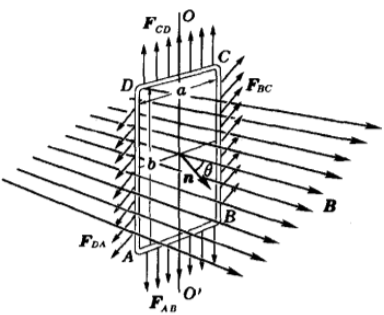
\includegraphics[width=\textwidth]{2-11.png}
    \caption{均匀磁场中矩形线圈所受力矩}
  \end{minipage}
  \hfill
  % 第二张图片
  \begin{minipage}[t]{0.3\textwidth}
    \centering
    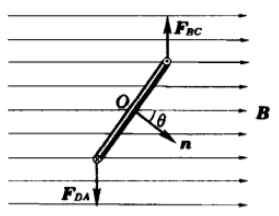
\includegraphics[width=\textwidth]{2-12.png}
    \caption{左图的投影图}
  \end{minipage}
  \hfill
  \begin{minipage}[t]{0.3\textwidth}
    \centering
    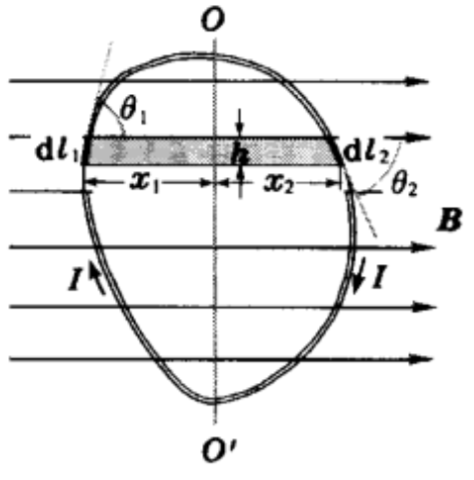
\includegraphics[width=\textwidth]{2-13.png}
    \caption{平面线圈在均匀磁场中受的力矩}
  \end{minipage}
\end{figure}

根据我们的图示,可以看出$AB$,$CD$两边所受的力对于轴线的力矩为$0$.对于$BC$,$DA$其受力大小均为$IbB$. 其力臂大小为:
$\frac{a}{2}\sin\theta$. 于是总的力矩大小为:
\[
L = 2IbB\cdot \frac{a}{2}\sin\theta = IabB\sin\theta = ISB\sin\theta = IS (\mathbf{n}\times \mathbf{B})
\]
最后这个结果其实对任意的平面载流线圈都是成立的,现在我们就来证明这一点。

我们把线圈分割为一系列垂直于转轴的小窄条,磁场对图示的两个电流元的作用力大小分别为:
\[
\d F_1 = I\d l_1 B\sin\theta_1 \;\d F_1 = I\d l_2 B\sin\theta_2
\]
几何关系告诉我们:
\[
\d l_1 \sin\theta_1 =\d l_2 \sin\theta_2 = \d h
\]
这两个力的合力矩为:
\[
\d L = IB\d h(x_1+x_2) = I B \d S
\]
于是积分可以得到总的力矩仍为$IBS$。注意到这里我们选取了磁感应强度平行于线圈平面,当不平行时,我们只需要使用叉乘将其重新投影到平行方向即可。

在证明过程中我们可以看到,$IS\mathbf{n}$是一个仅与载流线圈本身相关的矢量,我们定义这个量为线圈的磁矩,用$m$表示. 于是我们可以把力矩写成:
\[
\mathbf{L} = \mathbf{m} \times \mathbf{B}
\]

\clearpage

\chapter{磁介质}
\section{磁化强度和磁化电流}
我们曾经提到磁体具有吸引铁磁性物质的能力,并且将这种能力定义为磁性。事实上不仅仅是磁体和铁磁性物质具有磁性,其他物质或多或少都具有磁性。使物质具有磁性的物理过程称为磁化,而一切能够磁化的物质均称为磁介质。下面我们根据安培的分子电流假说,来介绍一些与磁介质相关的性质。

安培分子电流假说告诉我们,已磁化物质的磁性来源于物质内部有规则排列的分子电流。这里我们以软铁棒为例说明磁化的微观机制。
\insertfig{3-1.png}{磁化的微观机制}{0.25}

按照安培的观点,磁棒内每个磁``分子''(这里泛指磁介质中的微观基本单元)都相当于一个环形电流。在无外场的作用下,分子电流的取向是杂乱的,其磁矩相互抵消。这样宏观来看铁棒就不产生磁性。现在我们加入外加磁场$B_0$,称之为磁化场。在磁化场的力矩作用下,各分子环流的磁矩在一定程度上沿着场的方向排列起来,此时我们便说磁场被磁化了。

由图可以看出,在均匀介质均匀磁化的时候由于分子环流的回绕方向是一致的,在介质中任何两个分子环流中相邻的一对电流元方向总是彼此相反且抵消的,于是只有横截面边缘的各段电流元未被抵消。宏观看起来,这横截面内所有分子环流的总体效果与沿着截面边缘的一个大环形电流等效。

为了描述磁介质的磁化方向和程度,我们引
入磁化强度矢量的概念.
\begin{definition}[磁化强度矢量]
磁化强度矢量定义为单位体积内分子磁矩的矢量和,也即:
\[
\mathbf{M} = \frac{\sum_i \mathbf{m_i}}{\Delta V}
\]
\end{definition}

也正如电介质中极化强度矢量$P$与极化电荷之间有一定关系,磁介质中磁化强度矢量$M$与磁化电流之间也有一定的关系。

\begin{figure}[h]
  \centering
  % 第一张图片
  \begin{minipage}[t]{0.4\textwidth}
    \centering
    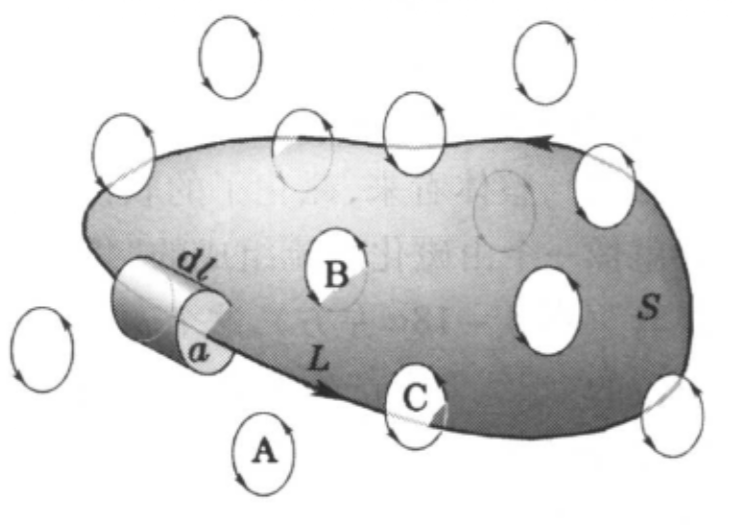
\includegraphics[width=\textwidth]{3-2.png}
    \caption{磁化强度与磁化电流的关系}
  \end{minipage}
  \hfill
  % 第二张图片
  \begin{minipage}[t]{0.4\textwidth}
    \centering
    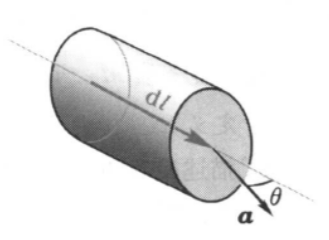
\includegraphics[width=\textwidth]{3-3.png}
    \caption{左图的微观截面}
  \end{minipage}
\end{figure}

为了方便解决问题,我们假定每个体积元内的分子磁矩都完全一致。设单位体积内的分子环流数为$n$,环内具有相同的电流$I$,环具有相同的面积$a$,于是介质中的磁化强度为
\[
M= nIa 
\]
我们在磁介质中划出一个宏观的面$S$来考察其有无分子电流通过。如图所示,我们只需要考虑图中仅与$S$一次相交的分子环流。首先我们取界面环线上的一个线元$\d \mathbf{l}$。以$\d \mathbf{l}$为轴线,$\mathbf{a}$为底面做一个柱体,其体积为$\d \mathbf{l}\cdot \mathbf{a}$.所有中心在此柱体内的分子环流都被$\d \mathbf{l}$穿过,每个分子环流贡献一个通过$S$面的电流$I$,于是$\d \mathbf{l}$穿过的所有分子环流总共贡献电流为
\[ n I \mathbf{a}\cdot \d \mathbf{l}=\mathbf{M}\cdot \d\mathbf{l}\]

于是我们得到磁化强度与磁化电流$I'$的分布有如下关系:
\[
\oint_L \mathbf{M}\cdot \d \mathbf{l} = \sum_{\text{L内}} I'
\]

为了得到磁化强度与介质表面磁化电流的关系,我们将上式应用于图示的回路。设此介质表面单位长度上的磁化电流为$i'$,则闯过矩形回路的磁化电流为$I'=i' \Delta l$,$M$的积分只在介质表面内的一边上不为$0$, 其贡献为$M_t\Delta l$从而得到:
\[
M_t \Delta l = l' \Delta l \Rightarrow M_t = i'
\]
考虑到方向,得到:
\[
i' = \mathbf{M} \times \mathbf{n}
\]

\insertfig{3-4.png}{磁化强度与表面磁化电流的关系}{0.25}

\section{磁介质中的磁场基本定理}
我们将产生磁化场的电流称为传导电流,与磁化电流相区别。如果已知磁介质的磁化强度分布,那么我们就可以根据前一节的内容确定介质内和表面的磁化电流分布。设由传到电流和磁化电流产生的磁感应强度分别是$\mathbf{B_0}$和$\mathbf{B'}$,则总磁感强度为二者之和,即:
\[
\mathbf{B} = \mathbf{B_0}+\mathbf{B'}
\]
这两种磁场都由毕奥-萨伐尔定律所决定,磁介质的全部作用在于提供磁化电流作为新的场源。显然$\mb{B}$应该满足真空中静磁场的高斯定理和安培环路定理:
\[
\oiint_S \mathbf{B} \cdot \d \mathbf{S} = 0
\]
\[
\oint_L \mathbf{B} \cdot \d \mathbf{l} = \mu_0\sum(I_0+I')
\]

也就是说磁介质中仍有高斯定理满足。由此,我们在两介质表面做一个柱形的高斯面,其底面分别位于两介质中。当所取高斯面厚度趋于$0$时,其侧面上的磁通量趋于$0$.于是上下底面的通量积分和为$0$.因为所取高斯面为柱面,上下底面面积相同,于是得到:
\[
B_{1n}=B_{2n}
\]
也即:\textbf{在介质表面磁感应强度法向连续。}

仿照电介质中我们引入辅助矢量消去极化电荷,我们同样可以引入一个辅助矢量来消去磁化电流。

\[
\oint_L \mathbf{B} \cdot \d \mathbf{l} = \mu_0\sum I_0+\mu_0\sum I'
\]
用磁化强度替换掉磁化电流:
\[
\oint_L \mathbf{B} \cdot \d \mathbf{l} = \mu_0\sum I_0+\mu_0 \oint_L M \cdot \d \mathbf{l}
\]
两边同除$\mu_0$,移项,得到:
\[
\oint_L (\frac{\mb{B}}{\mu_0}-\mb{M}) = \sum I_0
\]

于是我们引入:
\begin{definition}[磁场强度]
  

\[
\mathbf{H} = \frac{\mb{B}}{\mu_0}-\mb{M}
\]
称之为磁场强度。
\end{definition}
实验表明,对于各项同性的线性磁介质,磁化强度与磁场强度有简单正比关系:
\[
\mathbf{M} = \chi_m \mathbf{H}
\]

代入前式,我们得到:
\[
\mathbf{B} = \mu_0(1+\chi_m)\mathbf{H}
\]
取相对磁导率$\mu_r$和磁导率$\mu$:
\[
\mu_r = 1+\chi_m,\; \mu = \mu_0 \mu_r
\]
则在各向同性磁介质中,我们有:
\[
\mathbf{B} = \mu_0\mu_r \mathbf{H} = \mu \mathbf{H}
\]

处理磁介质问题的思路是与电介质类似的,利用我们已经知道分布的传导电流先求解相关量,最后给出相关的结果。下面看例题:
\begin{example}
  
一半径为$R_1$的长直导线上包裹着相对磁导率为$\mu_r$的磁介质,外半径为$R_2$。导线中通有电流$I$.求磁介质内部磁场的磁感应强度大小和磁介质界面处磁化电流的大小和方向。

首先由磁介质的安培环路定理:

\[
\oint_L \mathbf{H}\cdot \d \mb{l} = I \Rightarrow 2\pi r H = I (r>R_1) \Rightarrow H = \frac{I}{2\pi r} 
\]

由线性介质关系:
\[
B = \mu H = \frac{\mu_0\mu_r I}{2\pi r}, \; M = \chi_m H =\frac{(\mu_r-1) I}{2\pi r}
\]

由面电流密度与磁化强度的关系,内表面面磁化电流密度方向与传导电流相同:
\[
\alpha_1' = M_{in}  = \frac{(\mu_r-1) I}{2\pi r}
\]

内表面总的电流大小为:
\[
I_1' = 2\pi R\alpha_1' = (\mu_r-1) I
\]

同理,外表面面磁化电流密度与传导电流方向相反:
\[
\alpha_2' = M_{out}  = \frac{(\mu_r-1) I}{2\pi r}
\]

外表面总的电流大小为:
\[
I_2' = 2\pi R\alpha_2' = (\mu_r-1) I
\]
\end{example}


\section{磁介质的磁化规律和机理}
对于电介质来说,一般$\chi_e>0$。但磁介质的情况较电介质更加复杂。磁介质大致可以分类为顺磁质,抗磁质和铁磁质三种。对于顺磁质,$\chi_m>0$,对于抗磁质,$\chi_m<0$.

先来研究磁介质分子电流的微观机制。我们考虑电子绕核做半径为$r$的圆周运动。电子的角动量为
\[
L=\mathbf{r}\times m\mathbf{v}=mvr\hat{k}
\]
单位时间内通过轨道横截面的电量为电流,其大小为:
\[
I=\frac{ev}{2\pi r}
\]
于是因为轨道运动带来的磁矩为:
\[
\mathbf{m_{orb}} = I \cdot \pi r^2 -\hat{k} = \frac{1}{2}evr\hat{k}
\]
于是电子的轨道磁矩可以写为:
\[
\mathbf{m_{orb}}=\frac{e}{2m}\mathbf{L}
\]
一般我们定义磁矩与角动量的比值为旋磁比:
\[
\gamma_{orb}=-\frac{e}{2m}
\]

以上的磁矩由电子的轨道运动带来。电子同时具有一种叫做自旋角动的内禀性质,与电子的运动情况没有关系,是电子的固有属性。并且,自旋角动量找不到任何的经典运动对应,也就是说自旋角动量不仅并非电子绕着自身旋转带来的角动量,而且是一个纯粹的量子效应量。其旋磁比为:
\[
\gamma_{spin} = -\frac{e}{m}, m_{spin} = -\frac{e}{m}\mathbf{S}
\]
其中$S$是自旋角动量。

顺磁性物质的磁化机制大致可以描述如下:在外加磁场的作用下,原来因为热运动而完全随机取向的分子磁矩倾向于沿着磁场方向排列,从而产生沿着某方向的磁矩。然而由于热运动的存在,这种排列不可能完全整齐。外磁场越强,温度越低,排列越整齐,顺磁效应也就越强。顺磁物体分子磁矩有序排列之后产生的磁矩与外加磁场方向相同,该磁矩产生的磁场方向业也与外加磁场方向相同,于是宏观上看总磁场被增强。

根据上面的机制介绍,我们可以看出温度越高,顺磁效应越弱。同时当我们撤去外加磁场时,磁化会立刻消失。

抗磁性物质的磁化机制大致可以描述如下:在有外加磁场的情况下,电子轨道会感应出一个与外磁场反向的磁场,从而产生抗磁性。由此可见,抗磁性是普遍存在的。同时由于其由电子轨道运动引起,抗磁性通常非常弱,但不受温度影响。

在对抗磁物质施加外场时,其会受到力矩,并使电子的轨道运动角动量产生影响:
\[
\mathbf{M} = \mb{m_{orb}}\times \mathbf{B_0} \Rightarrow \d \mathbf{L} = \mathbf{M} \d t = (\mathbf{m_{orb}}\times \mb{B_0})\d t
\]
带入电子的磁矩与角动量之间的表达式,我们得到:
\[
\d \mathbf{L} = -\frac{e}{2m}(\mathbf{L}\times\mathbf{B_0}) \d t
\]
从而电子将以外磁场方向为轴产生进动。这种进动的结果类似于一个反向的环形电流,将产生一个反向的附加磁矩。

当然我们也可以从电子受力的角度对这一现象做些简单分析。设原子核带电为$Ze$,电子带电为$-e$,于是我们可以写出电子原有的运动方程:
\[
\frac{Ze^2}{4\pi\v_0r^2}=m\omega_0^2r
\]
加入外磁场后,电子受到的洛伦兹力为:
\[
\mathbf{F} = -e\bm{\omega}\times{\mathbf{r}}\times{\mb{B}} = e[\mb{B}(\bm{\omega}\cdot \mb{r})-\mb{r}(\bm{\omega}\cdot \mb{B})]=-e\mb{r}(\bm{\omega}\cdot \mb{B})
\]

对于$\omega$,$B$同向的情况,我们可以得到:
\[
\frac{Ze^2}{4\pi\v_0r^2}+e\omega rB=m\omega_0^2r
\]
取$\omega=\omega_0+\Delta \omega$,并且在磁场不大的情况下,有:
\[
\frac{Ze^2}{4\pi\v_0r^2}+e\omega rB +e\Delta \omega rB=m\omega_0^2r +2m\omega_0\Delta\omega+m(\Delta\omega)^2r
\]
两端第一项相消,第三项均略去,得到:
\[
\Delta \omega =\frac{eB}{2m}
\]
方向与$B$相同。

对于反向的情况,也会发现$\Delta \omega$与$B$方向相同。考虑到电子带负电,得到:
\[
\Delta m = \frac{er^2}{2}\Delta \omega =-\frac{e^2r^2}{4m}B
\]
新产生的磁矩与$B$的方向相反,带来抗磁效应。抗磁效应也会在撤去外电场后消失。

以上两种磁介质的磁性其实都很弱,它们的$|\chi_m|\ll 1$,而且往往都是常数。

对于铁磁体,$\mathbf{M}$和$\mathbf{H}$的关系不再一一对应,还与铁磁体的磁化历史有关。除此之外,铁磁体的磁化强度随外加磁场的变化还存在滞后性,称为磁滞效应。

对于铁磁质,其磁化强度往往远大于磁场强度,因此:
\[
B = \mu_0(H+M) \approx \mu_0 M
\]
也就是说,$B\sim H$曲线与$M\sim H$曲线相似。

下面我们介绍测定铁磁物体极化规律的方法。
\insertfig{3-5.png}{铁磁质的磁滞回线}{0.3}

我们取一块铁磁质,其从未被磁化,从$0$开始,逐步地增大铁磁体内的磁场强度$H$,这各过程在图纸中表现为$OS$,该曲线称起始磁化曲线。该曲线显示铁磁质在一开始的磁化过程中,磁感应强度$B$也会非线性地增大。在磁感应强度达到饱和之后,逐步减小磁场强度,其磁感应强度并不会沿着$SO$减小,而是会沿着$SR$曲线减小。当$H$减小到$0$时,磁感应强度并不减小到$0$。$R$点处对应的磁感应强度$B_R$称为剩余磁感应强度。进一步加入反向的磁场强度,当磁场强度达到$C$点对应值时,磁感应强度减小为$0$.$C$点对应的$H_C$称为矫顽力。继续反向增大$H$,磁感应强度沿着$CS'$曲线达到反向饱和,此后反向增大磁场强度,磁感应强度沿着$SS'$变化直到再次达到饱和,上述曲线称为磁滞回线。

铁磁质的磁性主要来源于电子的自旋磁矩,在没有外场的作用时,铁磁质中的电子自旋将在小范围内自发有序排列,形成一个个小的自发磁化区,这样的自发磁化区称为磁畴。量子力学理论告诉我们,这种自发磁化来源于电子之间的“交换作用”,使得电子自旋平行排列时能量更低。这种作用是纯量子效应,没有经典理论的对应。

在未磁化的铁磁质中,各磁畴内的自发的磁化方向不同,从而在宏观上不显示出磁性。在加外磁场后,起初磁化方向与磁化场方向相近的那些磁畴将会把临近的磁化方向与磁化方向相反磁畴的领域吞并一些,从而显示出宏观的磁性。当所有的磁畴都沿着磁化场的方向排列好时,介质磁化达到饱和。因此饱和磁化强度就等于每一个磁畴中原有的磁化强度。当所有磁畴中的元磁矩都完全排列好时,产生的磁化强度非常大。这就是铁磁质的磁性很强的原因。介质中的杂质和内应力在外场去掉后阻碍磁畴恢复原有状态,这导致了磁滞现象的产生。

\chapter{电磁感应}
\section{电磁感应定律}
在奥斯特发现电流的磁效应之后,人们致力于寻找其逆效应。然而,由于当时人们将探索的边界限制于静止的磁场,于是迟迟未能实现突破。直到法拉第用若干实验发现了电磁感应现象,并且由后人总结出其数学形式,形成了今天我们所见到的电磁感应定律。

在讨论电磁感应之前,我们先来看一下电动势。在一个电路中,当我们的电流在整个电路中不相同时,在某些地方会产生电荷的积累,这些积累的电荷产生的电场将会阻碍电流的流动,直到阻碍流动的电场与促进流动的电场到达平衡,从而建立起整个电路的平衡。也就是说,在驱动电流在整个电路中流动的过程中涉及到电源的非静电力和静电力。描述电池做功的能力时,我们常常用非经典力在整个回路中的线积分来描述($\mathscr C$也可以写作$\varepsilon$)
\[
\mathscr C = \oint_L  \mathbf{f_s} \cdot \d \mathbf{l}
\]
其中$f_s$是单位电荷所受的静电力

在理想电动势源中,电荷受到的合力为$0$。于是$E=-f_s$. 从而两板间的电势差为:
\[
V=-\int_a^b \mathbf{E} \cdot \d \mathbf{l} = \int_a^b f_s \cdot \d \mathbf{l} = \mathscr C
\]

法拉第曾经做了四个实验来验证他的猜想。我们简单总结一下:
\begin{itemize}
  \item 取一个与电流计相连的线圈,在其中插入和拔出磁棒时,电流计中有电流流过。
  \item 将上面的磁棒换为载流线圈,插入和拔出时,电流计中有电流流过。
  \item 将载流线圈插入线圈,控制开关使得载流线圈断电与通电,开关断开和闭合后电流计中有电流流过。
  \item 取一个平面线框,将其法线与磁场平行放置。拉动线框,其中有电流流过。
\end{itemize}

在这四个实验中,我们发现其共性是通过导线回路或者线圈的磁通量发生了变化。而且磁通量变化的越快,电流越大。

精确的实验表明:

\begin{theorem}[法拉第电磁感应定律]
导体回路中感应电动势的大小与穿过回路磁通量的变化率成正比。

\[
\mathscr C =\oint_L  \mathbf{f_s} =  \frac{\d \Phi}{\d t} =-\frac{\d}{\d t}\iint_S \mathbf{B} \cdot \d \mathbf{S}
\]

对于多匝线圈,我们需要将每一匝线圈的磁通都计算,若每匝线圈磁通都相同,有:

\[
\mathscr C = \frac{\d \Psi}{\d t} =-N\frac{\d \Phi}{\d t}
\]
\end{theorem}
其中$\Psi$被称为总磁通,也称磁通匝链数或磁链。


关于如何判断感应电流的方向,有楞次定律:
\begin{theorem}[楞次定律]
  闭合回路中感应电流的方向,总是使得它所激发的磁场来阻碍引起感应电流的磁通量的变化。
\end{theorem}
楞次定律其实是能量守恒的必然结果。感应电流在电路中流动时将释放焦耳热。这部分能量必然来源于克服斥力或者引力所做的机械功。否则插入磁棒的过程中感应电流既对外做功,又释放焦耳热,这显然是违反能量守恒的。

\section{动生电动势和感生电动势}
我们可以将产生电动势的原因简单分为两类。一种是在恒磁场中因为导体运动而产生感应电动势。另一种是导体不动,因为磁场的变化而产生感应电动势。前者被称为动生电动势,后者被称为感生电动势。

先介绍动生电动势。动生电动势可以被看作是洛伦兹力引起的。

\insertfig{4-1.png}{动生电动势与洛伦兹力}{0.25}

当导体以速度$v$向右运动时,导体内的自由电子也以速度$v$跟随运动。洛伦兹力的方向如图所示。则在洛伦兹力的推动下,自由电子将沿着$DCBA$方向运动,从而电流沿着$ABCD$方向。如果没有导体框与$CD$接触,那么自由电子将向$C$端聚集,从而使得$C$带负电,$D$带正电。此时我们可以把$C$端看成负极,$D$看成正极。这其中的非静电力就是作用在单位电荷上的洛伦兹力$\mathbf{v}\times\mathbf{B}$. 于是电动势为:
\[
\mathscr C = \int_C^D (\mathbf{v}\times \mathbf{B})\cdot \d \mathbf{l}
\]
事实上,我们可以对任意的一个线圈$L$计算电动势,上面的推导仍然适用。$L$可以闭合也可以不闭合,于是整个线圈中的电动势为:
\[
\mathscr C = \int_L (\mathbf{v}\times \mathbf{B})\cdot \d \mathbf{l}
\]
我们给出下面的证明。对于线圈上的一个线元$\d \mb{l}$,其在$\d t$时间内扫过的面积为$\d \mb{l} \times \mathbf{v} \d t$.

考虑原有的线圈所围成的曲面$S$和$\d t$时间后线圈所围成的曲面$S'$。这两个面和线圈扫过的侧面构成一整个闭合曲面。考虑磁场的高斯定理:
\[
\oiint \mb{B} \cdot \d \mathbf{S} =
-\iint_S \mb{B} \cdot \d \mathbf{S} +\iint_S' \mb{B} \cdot \d \mathbf{S}
+\oint_{L} \mb{B} \cdot (\d \mb{l} \times \mathbf{v}) \d t = 0
\]

前两项相减得到$-\d \Phi$,移项得到:
\[
-\d \Phi = -\oint_L \mathbf{B}\cdot (\d \mb{l}\times \mathbf{v}) \d t = \oint_L (\mathbf{v}\times \mathbf{B})\cdot \d \mathbf{l} \d t
\]
两边同时除以$\d t$

\[
\mathscr C = -\frac{\d \Phi}{\d t} =  \oint_L (\mathbf{v}\times \mathbf{B})\cdot \d \mathbf{l}
\]

我们考虑这样的一个例题:

\begin{example}
长度为$L$的一根铜棒,其一段在均匀磁场中以角速度$\omega$旋转,求这根铜棒两端的电势差。

铜棒旋转时切割磁感线,故棒两端之间有感应电动势。每个小段$\d l$产生的电动势方向相同,于是我们可以计算:
\[
V = \mathscr C = \int_0^L B\omega\d l =\frac{1}{2}B\omega L^2
\]

\end{example}
也许我们会有这样的问题,注意到洛伦兹力对电荷永不做功,这里我们又说动生电动势是由洛伦兹力做功引起的,这岂非矛盾?这种佯谬产生的原因是我们只计算了洛伦兹力的一部分。在运动导体中的电子不仅有导体本身的速度,还有相对导体的定向运动速度$u$,正是这种运动构成了感应电流。这个分量的方向恰好沿着$-\mb{v}$,阻碍导体运动,做负功阻碍导体的运动。因此洛伦兹力只是将外力克服洛伦兹力的一个分量所做的功通过另一个分量转化为感应电流的能量。

导体在磁场中运动产生动生电动势,其非静电力是洛伦兹力; 在磁场变化产生感生电动势的情形里非静电力是什么呢?实验表明,感生电动势完全与导体的种类和性质无关。这说明感生电动势是由变化的磁场本身引起的。

我们考虑一个固定的回路$L$,$S$为以$L$为边界的曲面。$Maxwell$提出变化的磁场会产生涡旋电场$\mathbf{E_i}$.产生感应电动势的非静电力就是涡旋电场,这也提示我们静电场与涡旋电场并非同一种电场,涡旋电场的环路积分不为$0$且恰好为感生电动势:
\[
\mathscr C = \oint_L \mathbf{E_i} \cdot  \d \mathbf{l} = -\frac{\d}{\d t} \iint_S \mathbf{B}\cdot \d \mathbf{S} = -\iint_S \frac{\partial \mathbf{B}}{\partial t}\cdot \d \mathbf{S}
\]
涡旋电场的存在是$Maxwell$电磁理论的基本假设之一。

现在我们来看一个感生电动势的应用——电子感应加速器。它的基本结构如图所示。

\begin{figure}[h]
  \centering
  % 第一张图片
  \begin{minipage}[t]{0.3\textwidth}
    \centering
    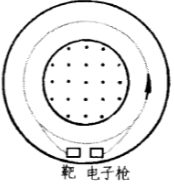
\includegraphics[width=\textwidth]{4-2.png}
    \caption{电子感应加速器}
  \end{minipage}
  \hfill
  % 第二张图片
  \begin{minipage}[t]{0.3\textwidth}
    \centering
    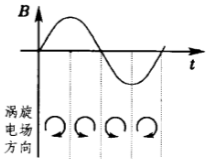
\includegraphics[width=\textwidth]{4-3.png}
    \caption{感应加速器中磁场变化位于不同相位时涡旋电场的方向}
  \end{minipage}
\end{figure}

在一个电流变化的周期内,只有四分之一的区间能够用于加速电子。这是因为,首先为了使电子得到加速,涡旋电场应该沿着顺时针方向,这要求第一或者第四个四分之一周期。其次为了使得电子不断加速,必须维持洛伦兹力指向圆心。可以看出,只有第一或者第二个四分之一周期。综上所述,只有第一个四分之一周期电子才能不断被加速。

为了实现这种加速,我们需要同时维持电子的圆周运动和加速。电子做圆形轨道时要求有向心力公式:
\[
evB = \frac{mv^2}{R} \Rightarrow mv = eBR \Rightarrow \d(mv) = eR\d B
\]

上式表明,只要电子动量随着磁感应强度成比例增加,就可以维持电子在轨道上运动。电子的加速过程可以描述如下:
\[
E_{orb} \cdot 2\pi R = -\frac{\d \Phi}{\d t} \Rightarrow 
E_{orb} = -\frac{1}{2\pi R}\frac{\d \Phi}{\d t}
\]
根据牛顿第二定律:
\[
\frac{\d (mv)}{\d t}=-eE_{orb}=\frac{e}{2\pi R}\frac{\d \Phi}{\d t} \Rightarrow \d(mv)  =\frac{e \d \Phi}{2\pi R}
\]
取$\overline{B}$为轨道内的平均磁感应强度,则有$\d \Phi = \pi R^2\d \overline{B}$. 于是我们得到:
\[
\d B = \frac{1}{2}\d \overline{B} \Rightarrow B = \frac{1}{2}\overline{B}
\]
也就是说,当轨道处磁感应强度为轨道内磁感应强度的一半时,电子能够在稳定的轨道上被加速。

最后我们简单介绍趋肤效应。当导线通入稳恒电流时,横截面上的电流密度基本上是均匀分布的。然而当导线通入交变电流时,将会激发出磁场。这一变化的磁场又会激发出涡旋电场,从而产生涡电流。在导线表面,涡电流的方向与传导电流相同,在靠近轴线处反之。导线中的电流趋向于分布在导线的表面,这一效应被称为趋肤效应。

\section{自感与互感}
\insertfig{4-4.png}{两线圈之间的互感}{0.3}
当线圈$1$中的电流变化时所激发的变化磁场,会在它邻近的另一线圈$2$中产生感应电动势; 同样线圈$2$中的电流变化时也会在线圈$1$中产生感应电动势。这种现象称为互感现象,产生的感应电动势称为互感电动势。显然一个线圈中的互感电动势不仅与另一线圈中的电流变化率有关,而且也与两个线圈的结构以及它们之间的相对位置有关。

设线圈$1$所激发的磁场通过线圈$2$的磁链为$\Psi_{12}$按照毕奥-萨伐尔定律,$\Psi_{12}$与线圈$1$中的电流$I_1$成正比:
\[
\Psi_{12} = M_{12} I_1
\]
对称地,我们有:
\[
\Psi_{21} = M_{21} I_2
\]

其中的$M_{12},M_{21}$被称为互感系数,简称互感。可以证明$M_{12}=M_{21}=M$。当然这里我们讨论的过程中不涉及到铁磁质,否则$M_{12},M_{21}$都不再是常数。

当电流$I_1$发生变化时,将在线圈$2$中激发的感应电动势为:
\[
\mathscr C_1 = -\frac{\d \Psi_{12}}{\d t} = -M\frac{\d I_1}{\d t}, \mathscr C_2 = -\frac{\d \Psi_{12}}{\d t} = -M\frac{\d I_2}{\d t}
\]
上面我们已经假定互感系数保持不变。

同样地,当一个线圈中通入电流时,线圈会产生磁场。这一磁场对线圈自身是有磁通量的。因此当线圈内部的电流发生变化时,变化的磁场自然也会导致穿过线圈的磁通发生变化。于是线圈中将产生感应电动势,这一现象被称为自感现象。一个线圈便可以称为一个自感。

我们知道线圈中电流所激发的磁感应强度与电流成正比,因此通过线圈的磁链也正比于线圈中的电流,即:
\[
\Psi = LI \Rightarrow \mathscr C = -L\frac{\d I}{\d t}
\]
$L$被称为自感系数。同样地,不存在铁磁质的情形下,自感系数则为常数。

我们来考虑一个截面积为$S$,长为$l$的$N$匝长直密绕螺线管的自感系数。设该螺线管上的电流大小为$I$. 则其产生的磁感应强度大小为:
\[
B = \mu_0\frac{NI}{l}
\]
通过螺线管横截面的磁通量为$\Phi= BS=\mu_0\frac{NIS}{l}$。于是自感系数为:
\[
L =\frac{N\Phi}{I}=\mu_0\frac{N^2S}{l} = \mu_0 n^2 V
\]

两个线圈之间的互感系数与各自的自感系数有一定的联系。当两个线圈中每一个线圈所产生的磁通量对于每一匝来说都相等,并且全部穿过另一个线圈的每一匝。这种情况就被称为无漏磁。一般而言,通过自身回路的磁通量要大些。
\[
\Phi_{21} = k_1 \Phi_1, \;\Phi_{12} = k_2 \Phi_2, k_1\le 1, k_2\le 1
\]

考虑到先前的定义,我们可以把磁链写成:
\[
\Psi_{21} = N_2 \Phi_{21} = N_2 k_1 \Phi_1,\; \Psi_{12} = N_1 \Phi_{12} = N_1 k_2 \Phi_2
\]

因此互感系数满足:
\[
M_{21}=\frac{N_2k_1\Phi_1}{I_1},\;M_{12}=\frac{N_1k_2\Phi_2}{I_2}\Rightarrow M^2 =\frac{N_1N_2k_1k_2\Phi_1\Phi_2}{I_1I_2}
\]

考虑自感关系,有:
\[
\Psi_1 = N_1 \Phi_1 = L_1 I_1,\;\Psi_2 = N_2 \Phi_2 = L_2 I_2
\]

把上式代入,得到:
\[
M = \sqrt{k_1k_2}\sqrt{L_1L_2}
\]

$k=\sqrt{k_1k_2}$被称为线圈$1$和线圈$2$之间的耦合系数。

若不存在漏磁,则$k=1$:
\[
M=\sqrt{L_1L_2}
\]

\section{\texorpdfstring{暂态过程\, 磁场能量}{暂态过程 磁场能量}}
暂态过程指的是是电路状态从一种稳态转变为另一种稳态时所经历的过渡过程。这种暂态过程通常在电路发生突变,比如开关闭合,电源接入,初始条件发生变化时。电路状态改变时,电容,电感等元件需要时间来调整其储存的能量。这就产生了暂态过程。

我们来看一个电路,将所有的电容,电阻,电感分别等效为$C,R,L$三个基本元件,设初态$t=0$时电路中$I=0$,电容极板上电荷$q=0$. 于是我们可以写出回路中的电势降方程:
\[
L\frac{\d I}{\d t}+\frac{q}{C}+IR = \v
\]
注意到:$I=\frac{\d q}{\d t}$,可以整理我们的方程为:
\[
L\frac{\d^2 q}{\d t^2}+R\frac{\d q}{\d t}+\frac{q}{C}=\v
\]

我们讨论一下几种特殊情况的电路:

(1)$L=0$.这是一个$RC$电路。解上述方程,可以得到:
\[
q =\v C(1-e^{-\frac{t}{RC}}),\; I=\frac{\v}{R} e^{-\frac{t}{RC}}
\]
其中$\tau=RC$被称为特征时间,可以用来描述电路达到稳态的时间长短。我们可以看到,在充电的过程中,电容上的电量逐步从$0$开始增加,最终达到饱和。而电流则以指数衰减为$0$.

放电时,取$\v=0$电量和电流大小都以指数形式衰减:
\[
q = q_0e^{-\frac{t}{RC}},\; I = -\frac{q_0}{RC}e^{-\frac{t}{RC}}
\]
其中$q_0$是初始状态下电容上的电量。

(2)$C=0$.这是一个$RL$电路。解上述方程,可以得到:
\[
I =\frac{\v}{R}(1-e^{-\frac{R}{L}t})
\]
其中$\tau=\frac{L}{R}$为特征时间

这个解表明,在初始状态下,电流为$0$.后电流逐步以指数增长形式达到稳态。放电过程与之恰好相反:
\[
I = I_0 e^{-\frac{L}{R}t}
\]

在以上的讨论中,我们发现电容上的电压和电荷不能瞬间变化,电感中的电流不能瞬间变化。否则会产生无穷大电动势。

(3)$R$=0.这是一个$LC$电路。解上述方程,我们得到:
\[
q=q_0\cos(\omega_0 t+\phi),\quad \omega_0 = \frac{1}{\sqrt{LC}}
\]
也就是说,在这种电路中电荷和电流都将以余弦形式震荡,形成我们后面会讨论的产生电磁波的物质基础。

(4)一般情况。这时候,我们把整个方程化为标准的二阶常系数微分方程:
\[
\frac{\d^2 q}{\d t^2}+2\beta \frac{\d q}{\d t}+\omega_0^2 q = \v,\quad \beta = \frac{R}{2L}, \quad \omega_0 = \frac{1}{\sqrt{LC}}
\]

这方程的通解与$RLC$的具体数值有关,我们可以定义阻尼度:
\[
\lambda = \frac{R}{2}\sqrt{\frac{C}{L}}
\]

$\lambda<1$为欠阻尼, $\lambda=1$为临界阻尼,$\lambda>1$为过阻尼。欠阻尼情况下,电路的振荡频率为:
$\omega = \sqrt{\frac{1}{LC}-(\frac{R}{2L})^2}$.上述方程的一个特解是$q=\v C$.

讨论了暂态过程,我们现在来看一下磁场中的能量。我们考虑在一个线圈中建立电流的过程。当线圈与电源接通时,由于自感的存在的,电路中的电流$i$并不立刻变化到稳定值$I$。在这一变化过程中,电路中外电源的电动势不仅要供给电路中的焦耳热,而且要反抗自感电动势的做功,这部分反抗自感电动势所做的额外的功应当以能量的形式储存在线圈中。

$\d t$时间内,电源的电动势反抗自感电动势做功为:
\[
\d A = -\mathscr C_{L} i \d t =-(-L\frac{\d i}{\d t})\d t = Li\d i
\]
因而在整个建立电流的过程中,电源的电动势反抗自感电动势所做的功为:
\[
A = \int_0^I Li\d i =\frac{1}{2}LI^2
\]
当切断电源时,电流由稳定值$I$减少到$0$.线圈中产生了与电流方向相反的自感电动势。线圈中原本存储的能量将会以同样的形式释放出来。于是我们便说,自感线圈将会存储磁能,在一个自感系数为$L$的线圈中建立强度为$I$的电流,线圈中存储的能量是$\frac{1}{2}LI^2$.这被称为自感磁能。

下面简单讨论互感磁能:我们考察在相邻的线圈$1$和$2$中建立电流的过程中抵抗互感电动势所做的功:

\[
A = -\int_0^{\infty}\mathscr C_{21}i_1\d t-\int_0^{\infty}\mathscr C_{12}i_2\d t =\int_0^{\infty} M(i_1\frac{\d i_2}{\d t}+i_2\frac{\d i_1}{\d t})=M\int_0^{\infty}\frac{\d(i_1i_2)}{\d t} \d t = MI_1I_2
\]
也就是说线圈中存储的互感能量为$MI_1I_2$.

我们从螺线管入手导出磁场能量的一般形式:考虑螺线管的磁导率为$\mu$ 长度为$l$,截面积为$S$,线圈匝数为$N$,电流强度为$I$,则环内磁场为:
\[
B  =\mu nI
\]
螺线管的自感系数在之前已经推导过:
\[
L = \frac{\mu S^2}{l} = \mu n^2 V
\]
于是螺线管储存的磁能为:
\[
W_m = \frac{1}{2}LI^2 = \frac{1}{2}\mu n^2 I^2 V = \frac{1}{2}VBH
\]
于是螺线管内的磁能密度为:
\[
w_m = \frac{1}{2}\mathbf{B}\cdot \mathbf{H}
\]
上式对于一般的磁场也成立。这个式子的建立可以与我们建立电场能量公式的过程类比。

\chapter{Maxwell电磁理论}
\section{Maxwell电磁理论的建立}
在我们前面的所有讨论结束之后,似乎电磁学已经被我们穷尽了。对于静电场和静磁场,我们有相应的高斯定理和环路定理,理论上已经可以确定一切电场和磁场的具体形式。对于导体和电磁介质,虽然还有一些问题不那么好理解,但基于Lorentz的经典电子论,也获得了比较令人满意的结果。那么还有什么需要我们研究的吗?现在我们所面临的状态,恰与Maxwell\footnote{这个名字不能不使人浮想联翩——Max well,这一电磁理论确实可算作经典物理中的最精妙理论。}开始他的研究之前的状态十分类似。

在我们正式讨论Maxwell的想法之前,我们先补充一下之前没有详细讨论过的边界条件。

\begin{figure}[h]
  \centering
  % 第一张图片
  \begin{minipage}[t]{0.4\textwidth}
    \centering
    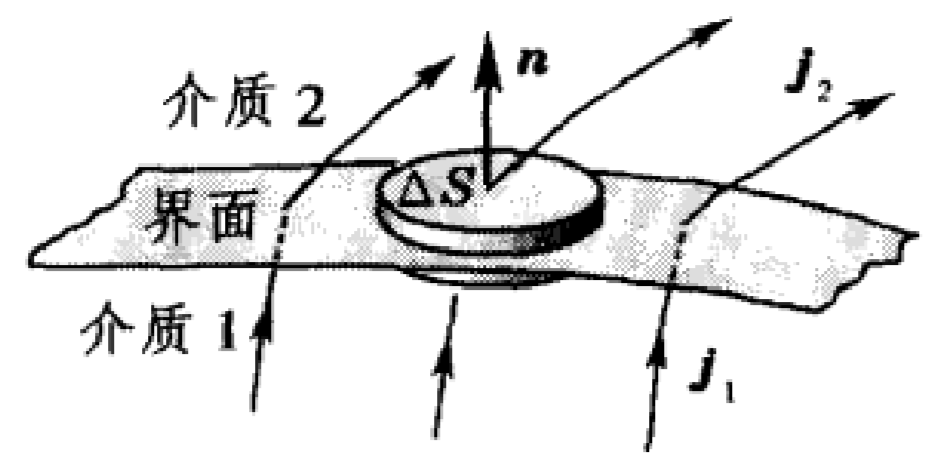
\includegraphics[width=\textwidth]{5-1.png}
    \caption{法向分量的连续性}
  \end{minipage}
  \hfill
  % 第二张图片
  \begin{minipage}[t]{0.4\textwidth}
    \centering
    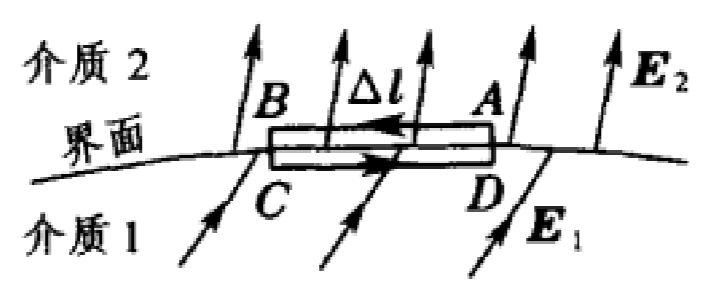
\includegraphics[width=\textwidth]{5-2.png}
    \caption{切向分量的连续性}
  \end{minipage}
\end{figure}

考虑两个电介质界面:我们取一个面元$\Delta S$,以其为底面作一个柱形高斯面,考虑通过这个高斯面的电位移通量,根据高斯定理: 
\[
\oiint \mb{D} \cdot \d \mathbf{S} = \iint_{S_1+S_2+S_{\text{侧}}} \mathbf{D}\cdot \d S = \sigma_f
\]
其中$\sigma_f$为自由电荷面密度。侧面积趋于$0$,其通量也趋于$0$,在$1,2$上的通量分别为:$-\mb{D_1}\cdot \mb{n} \Delta S$,$\mb{D_2}\cdot \mb{n} \Delta S$

于是我们得到:
\[
(D_1-D_2) \cdot n = \sigma_f
\]

一般而言,我们讨论的界面上都没有自由电荷分布。于是我们得到:
\[
D_{1n}=D_{2n}
\]
也就是说:在边界面两侧电位移矢量法向分量连续。

取矩形闭合环路$ABCDA$,其中$AB=CD=\Delta l$.考虑$E$沿着此闭合环路的线积分:
\[
\oint \mb{E} \cdot \d \mb{l} = \int_A^B \mb{E} \cdot \d \mb{l}+ \int_B^C \mb{E} \cdot \d \mb{l}+\int_C^D \mb{E} \cdot \d \mb{l}+\int_D^A \mb{E} \cdot \d \mb{l}=0
\]
注意到$BC$和$DA$的长度相较于$AB$和$DC$为高阶无穷小,在其上的积分为$0$
.在$AB$和$DC$上两侧的积分分别为:$-E_{1t}\Delta l$和$E_{2t}\Delta l$于是我们得到:
\[
E_{1t} = E_{2t}
\]
这就是电介质分界面上的第二个边界条件,它表明边界面两侧电场强度的切向分量连续。

对于磁介质界面,我们只需要把$D$替换为$B$,就可以得到法向连续; 把$E$替换为$H$
并且假设没有传导电流,就得到了切向连续。

总结起来就是,在介质界面上没有自由电荷或者传导电流的时候:

(1)电位移矢量$D$,磁感应强度矢量$B$的法向分量连续;

(2)电场强度矢量$E$,磁场强度矢量$H$的切向分量连续。

下面我们就来介绍Maxwell的工作。Maxwell时代的电磁场基本规律可以概括如下:

由库仑定律和场强叠加原理可以得出静电场的两条定理:

(1)静电场的高斯定理
\[
\oiint \mathbf{D} \cdot \d \mathbf{S} = q_0
\]

(2)静电场的环路定理
\[
\oint \mb{E}\cdot \d \mb{l} = 0
\]

由毕奥-萨伐尔定律可以得出恒磁场的两条重要定理:

(3)磁场的高斯定理
\[
\oiint \mathbf{B} \cdot \d \mb{S} = 0
\]

(4)安培环路定理
\[
\oint \mb{H} \cdot \d \mb{l} = I_0
\]

(5)此外还有法拉第发现的磁场变化时的规律:
\[
\mathscr C = -\frac{\partial \Phi_B}{\partial t}
\]

我们先介绍电流密度的概念。先前我们已经介绍过电流强度的定义。电流强度被定义为单位时间内通过所考察的横截面的电量。这告诉我们可以定义电流的密度:
\[
I = \iint \mb{j}\cdot \d \mb{S} 
\]
其中$j$被称为电流密度。

此外还有容易被忽视的电荷守恒原理。对于一个闭合曲面,其所包裹电荷的变化率加上流经该表面的电流强度应该为$0$,于是我们得到

(6)电荷守恒原理:
\[
\oiint j_0 \cdot \d \mb{S} +\frac{\d q_0}{\d t}= 0
\]
在前面我们已经提到过Maxwell发现感应电动势现象预示着变化的磁场周围会产生涡旋电场,因此法拉第电磁感应定律预示着在普遍情形下电场的环路定理应该写为:
\[
\oint_L \mb{E} \cdot \d l = \iint_S -\frac{\partial \mb{B}}{\partial t} \cdot \d \mb{S}
\]
静电场环路定理应当是它的一个特例。

Maxwell从当时的实验和理论分析中都没有发现电场的高斯定理有什么问题,于是Maxwell假定它们在普遍情形下仍然成立。然而Maxwell在分析安培环路定理时发现了将其应用到非恒定情形下时遇到了矛盾。

我们可以改写一下我们的安培环路定理:
\[
\oint_L H \cdot \d \mb{l} = I_0 = \iint_S \mb{j_0} \cdot \d \mb{S} 
\]

现在我们想问,非恒定条件下安培环路定理是否仍然成立?想要上式有意义的话,就必须要求穿过任意以$L$为边界的曲面的传导电流都相等,也就是说:
\[
\iint_S \mb{j_0} \cdot \d \mb{S_1} = \iint_S \mb{j_0} \cdot \d \mb{S_2} \equiv \oiint_S  \mb{j_0} \cdot \d \mb{S} =0 
\]
其中$S_1$,$S_2$是两个以$L$为边界的不同曲面。恒定情况下,上式的正确性由电荷守恒原理保证。

\insertfig{5-3.png}{非恒定情况下安培定理的矛盾}{0.25}

但非恒定情况下上式不成立。我们考虑这样的一个电容器的充放电电路。我们取$S_1$与导线相交,$S_2$穿过电容器的两极板之间,则穿过$S_1$的电流不为$0$,而穿过$S_2$的电流为$0$.这样上面的式子就失去了意义。如何解决这个矛盾呢?

我们需要回到我们没有使用过的电荷守恒原理:
\[
\oiint_S j_0 \cdot \d \mb{S} = -\frac{\d q_0}{\d t}
\]
注意到高斯定理为我们提供了一种计算自由电荷的方法:
\[
\oiint \mathbf{D} \cdot \d \mathbf{S} = q_0
\]
从而:
\[
\frac{\d q_0}{\d t} = \frac{\d}{\d t}\oiint_S \mb{D} \cdot \d \mb{S} = \oiint_S \frac{\partial \mb{D}}{\partial t} \cdot \d \mb{S} 
\]
这样我们可以改写电荷守恒方程:
\[
\oiint_S j_0 \cdot \d \mb{S} = -\oiint_S \frac{\partial \mb{D}}{\partial t} \cdot \d \mb{S} \Rightarrow \oiint_S (\mb{j_0}+\frac{\partial \mb{D}}{\partial t})\cdot \d \mb{S} = 0
\]
这样我们发现$\mb{j_0}+\frac{\partial \mb{D}}{\partial t}$这个量始终是保持连续的。仿照磁通量,我们可以定义电位移通量:
\[
\Phi_D = \iint \mb{D} \cdot \d \mb{S} \Rightarrow \frac{\d \Phi_D}{\d t} = \iint \frac{\partial \mb{D}}{\partial t}\cdot \d \mb{S}
\]

Maxwell把$\frac{\partial \mb{D}}{\partial t}$称为位移电流,$\frac{\partial \mb{D}}{\partial t}$被称为位移电流密度,位移电流与传导电流合在一起称为全电流。全电流在任意情况下都是连续的。

上述假设被称为位移电流假设。位移电流的引进虽然不存在逻辑上的矛盾,但是其正确与否仍然有待进一步的实验事实来证明。

这样非恒定情况下,我们应该用全电流代替不具有连续性的传导电流,这样我们可以修改安培环路定理:
\[
\oint \mb H \cdot \d \mb{l} = \iint_S (\mb{j_0}+\frac{\partial \mb{D}}{\partial t})\cdot \d \mb{S}
\]

为了正确地理解位移电流的实质,我们利用$\mb = \v_0 \mb{E} + \mb{P}$把位移电流分为两部分:
\[
j_d = \v_0 \frac{\partial \mb{E}}{\partial t}+\frac{\partial \mb{P}}{\partial t}
\]

式子中的第一项与电场强度随时间的变化率有关,即使在真空中也存在; 第二项是极化强度的变化引起,而极化强度的变化正式分子内部的束缚电荷的微观运动所引起的。事实上分子电流定向排列形成的磁化电流也是束缚电荷的微观运动所引起的。传导电流,极化电流和磁化电流显然是可以激发电场的。然而,最基本的第一项完全由于电场变化产生,与电荷的运动无关。

因此Maxwell的位移电流假设的实质是:随时间变化的电场和电流会激发磁场。而我们先前所做的涡旋电场假设,其实质是随时间变化的磁场会激发电场。这两个假设共同作用,就暗含着电磁场会在空间中以波动形式传播的结论。这正是Maxwell的第一个成功预言。

\insertfig{5-4.png}{变化的电磁场自源出发向四周传播形成电磁波}{0.25}

现在,我们已经完成了所有的工作,我们现在给出总结:

\textbf{Maxwell 方程的积分形式}
\begin{align*}
\oiint_{S} \mathbf{D}\cdot \d\mathbf{S} &= \iiint_{V} \rho_f\,\d V, \\[4pt]
\oiint_{S} \mathbf{B}\cdot \d\mathbf{S} &= 0, \\[4pt]
\oint_{L} \mathbf{E}\cdot \d\mathbf{l} &= -\frac{d}{dt}\iint_{S}\mathbf{B}\cdot \d\mathbf{S}, \\[4pt]
\oint_{L} \mathbf{H}\cdot \d\mathbf{l} &= \iint_{S}\mathbf{J_f}\cdot \d\mathbf{S}
+ \frac{d}{dt}\iint_{S}\mathbf{D}\cdot \d\mathbf{S}.
\end{align*}

数学上,我们有Gauss 散度定理与 Stokes 旋度定理(对足够光滑的矢量场$\mb{F}$):
\begin{align*}
\iiint_{V} (\nabla\cdot\mathbf{F})\,\d V &= \oiint_{S} \mathbf{F}\cdot \d\mathbf{S}, \\[4pt]
\iint_{S} (\nabla\times\mathbf{F})\cdot \d\mathbf{S} &= \oint_{L} \mathbf{F}\cdot \d\mathbf{l}.
\end{align*}

利用上述公式,我们可以得到:
\begin{align*}
\iiint_{V} (\nabla\cdot\mathbf{D})\,\d V &= \oiint_{S} \mathbf{D}\cdot \d\mathbf{S} = \iiint_{V} \rho_f\,\d V, \\[4pt]
\iint_{S} (\nabla\times\mathbf{E})\cdot \d\mathbf{S} &= \oint_{L} \mathbf{E}\cdot \d\mathbf{l}  =-\iint_S \frac{\partial \mathbf{B}}{\partial t}\cdot \d \mathbf{S}.\\[4pt]
\iiint_{V} (\nabla\cdot\mathbf{B})\,\d V &= \oiint_{S} \mathbf{B}\cdot \d\mathbf{S} = 0, \\[4pt]
\iint_{S} (\nabla\times\mathbf{H})\cdot \d\mathbf{S} &= \oint_{L} \mathbf{H}\cdot \d\mathbf{l} = \iint_S (\mb{j_0}+\frac{\partial \mb{D}}{\partial t})\cdot \d \mb{S}.
\end{align*}

注意到上面的四个式子要求对于任意的曲面和其包裹的空间均成立,我们得到;

\textbf{Maxwell 方程的微分形式}
\begin{align*}
\nabla\cdot\mathbf{D} &= \frac{\rho_f}{\varepsilon_0}, \\[4pt]
\nabla\cdot\mathbf{B} &= 0, \\[4pt]
\nabla\times\mathbf{E} &= -\frac{\partial\mathbf{B}}{\partial t}, \\[4pt]
\nabla\times\mathbf{H} &= \mathbf{J_f} + \frac{\partial\mathbf{D}}{\partial t}.
\end{align*}

对于电磁介质,我们还需要相关的描述介质的方程式,一般被称为本构方程。对于各向同性线性介质:
\begin{align*}
\mathbf{D} &= \v_r\varepsilon_0 \mathbf{E}, \\[4pt]
\mathbf{B} &= \mu_r\mu_0 \mathbf{H}, \\[4pt]
\mathbf{J} &= \sigma \mathbf{E}.
\end{align*}

到这里,我们已经完成了所有的工作。我们以Maxwell方程为最终形式,完成了经典电磁场理论。如果你坚持学习到现在并掌握了前面的内容,那么恭喜你,你已经基本上学会了求解电磁学问题所需要的所有理论基础。剩下的无非是一些特殊的数学技巧,如多极展开,分离变量法,镜像法之类。它们大多是数学理论在电磁学的具体应用。

这里当然是一个合适的终点(并非考试意义上的终点!),但从另一个意义上说我们刚好到达了起点,可以开始充分享受电磁场理论的威力和其丰富内容。下一节内容——电磁波将会是我们应用电磁场理论的开始,也是历史上Maxwell理论的最重要应用。
\begin{center}
  \textbf{无论如何,再次恭喜你看到了这里!}
\end{center}

\section{电磁波}
对于无自由电荷和传导电流的各向同性均匀线性介质空间,则这些空间中有:
\begin{align*}
\nabla\cdot\mathbf{D} &= \nabla\cdot\mathbf{E} =0, \\[4pt]
\nabla\cdot\mathbf{B} &= \nabla\cdot\mathbf{H}= 0, \\[4pt]
\nabla\times\mathbf{E} &= -\mu_r\mu_0\frac{\partial\mathbf{H}}{\partial t}, \\[4pt]
\nabla\times\mathbf{H} &= \v_r\v_0\frac{\partial\mathbf{E}}{\partial t}.
\end{align*}

我们考虑Maxwell方程中这个方程:
\begin{align*}
\nabla\times\mathbf{E} &= -\mu_r\mu_0\frac{\partial\mathbf{H}}{\partial t}
\end{align*}

数学上,我们有这样的矢量分析公式:
\[
\nabla \times  (\nabla \times \mb{E}) = \nabla(\nabla \cdot \mb{E})-\nabla^2 \mb{E}
\]

对该式两边求旋度,左侧得到:
\[
\nabla \times (\nabla \times \mb{E})= \nabla(\nabla \cdot \mb{E})-\nabla^2 \mb{E} = -\nabla^2 E
\]
这里利用了$\nabla\cdot\mathbf{E} =0$. 右侧得到:
\[
\nabla \times (-\mu_r\mu_0\frac{\partial\mathbf{H}}{\partial t}) = -\mu_r\mu_0\frac{\partial}{\partial t} (\nabla \times \mathbf{H}) = -\mu_r\mu_0\v_r\v_0 \frac{\partial^2 \mb{E}}{\partial t^2}
\]
两边相等,整理得到:
\[
\frac{\partial^2 \mb{E}}{\partial t^2} - \frac{1}{\mu_r\mu_0\v_r\v_0} \nabla^2 \mb{E} = 0
\]
同样的方法,我们可以得到:
\[
\frac{\partial^2 \mb{H}}{\partial t^2} - \frac{1}{\mu_r\mu_0\v_r\v_0} \nabla^2 \mb{H} = 0
\]

数学理论告诉我们,上述形式的微分方程被称为三维波动方程。上述方程的一种解的形式是:
\begin{align*}
\mb{E} &= \mb{E_0} \cos(\omega t - \mathbf k \cdot \mathbf r), \\[4pt]
\mb{H} &= \mb{H_0} \cos(\omega t - \mathbf k \cdot \mathbf r)
\end{align*}


我们取$v=\frac{1}{\sqrt{\mu_r\mu_0\v_r\v_0}}$为电磁波的波速,则上述方程同时应满足色散关系:
\[
\omega = vk
\]

注意到真空中,电磁波的波速为:
\[
c= \frac{1}{\sqrt{\v_0\mu_0}}
\]
于是我们可以定义折射率:
\[
n = \frac{v}{c} = \sqrt{\mu_r\v_r}
\]

这正是Maxwell从电磁波理论出发,对光学所做的一些初步研究。对于一般的材料,$\mu_r\approx 1$. 于是我们可以近似认为:
\[
n = \sqrt{\v_r}
\]

现在我们已经研究清楚了电磁波具有的一般形式。下面让我们来看平面电磁波.平面电磁波中,
\begin{align*}
\mb{E} &= \mb{E_0} \cos(\omega t - \mathbf k \cdot \mathbf r), \\[4pt]
\mb{H} &= \mb{H_0} \cos(\omega t - \mathbf k \cdot \mathbf r)
\end{align*}
$\mb{E_0},\; \mb{B_0}$都是常矢量。

我们对$\mb{E}$求散度,计算得到:
\[
\nabla \cdot \mb{E} = \mb{E_0} \cdot \nabla(\cos(\omega t -\mb{k}\cdot \mb{r})) = sin(\omega t- \mb{k}\cdot \mb{r})\mb{k}\cdot \mb{E_0}
\]

注意到空间中无电荷存在,$\nabla \cdot \mb{E}=0$,于是:
\[
\mb{k}\cdot \mb{E_0} = 0
\]
这说明波矢$\mb{k}$和电场强度矢量$E$垂直。同理可以证明$\mb{k}$与磁场强度矢量$\mb{H}$也垂直。

因此平面电磁波的电场方向与磁场方向都与波的传播方向垂直,因此我们说平面电磁波是横波。

现在我们对$\mb{E}$求旋度,计算得到:
\[
\nabla\times\mb{E} =  \nabla(\cos(\omega t -\mb{k}\cdot \mb{r}))\times \mb{E_0} = \sin(\omega t- \mb{k}\cdot \mb{r})\mb{k}\times \mb{E_0}
\]

假定磁场强度与电场强度的变化存在相位差$\varphi$,则磁场强度矢量应该具有形式:$\mb{H} = \mb{H_0} \cos(\omega t - \mathbf k \cdot \mathbf r+\varphi)$ 根据Maxwell方程,我们得到:
\[
\sin(\omega t- \mb{k}\cdot \mb{r})\mb{k}\times \mb{E_0}= \nabla \times \mb{E} = -\mu_r\mu_0\frac{\partial\mathbf{H}}{\partial t} = \mu_0 \mu_r \omega \mb{H_0}sin(\omega t- \mb{k}\cdot \mb{r}+\varphi)
\]

为了使上式始终成立,必须要求$\varphi = 0$. 同时有:
\[
\mb{k} \times \mb{E_0} = \mu_0\mu_r \omega \mb{H_0} 
\]
注意到平面电磁波中$\mb{E_0}$与$\mb{E}$同向,$\mb{H_0}$与$\mb{H}$同向向。
则由上面这个结果,我们看出$\mb{k},\mb{E},\mb{H}$三者两两垂直。

考虑到色散关系$\omega = vk$,化简上式得到:
\[
\frac{E}{H} = v\mu_r\mu_0 = \sqrt{\frac{\mu_r\mu_0}{\v_r\v_0}}
\]
\[
\frac{E}{B} =  \sqrt{\frac{1}{\mu_r\mu_0\v_r\v_0}} = v
\]

现在我们总结一下平面电磁波的基本性质:
\begin{itemize}
  \item $\mb{E}$和$\mb{B}$都与电磁波的传播方向垂直,电磁波是横波;
  \item $\mb{E}$和$\mb{B}$相互垂直,且$\mb{E}\times\mb{B}$总是沿着传播方向$\mb{k}$的;
  \item $\mb{E}$和$\mb{B}$之间没有相位差;
  \item $\frac{E}{B}=v$,$v=\frac{1}{\sqrt{\v_r\mu_r\v_0\mu}}$
\end{itemize}


下面我们介绍一下振荡偶极子电磁波。振荡电偶极子是电磁辐射的基本源之一,尤其是在天线和微观粒子中。这种电磁波一般源于一个电偶极矩以余弦形式变化的电偶极子:

\[
p = ql_0\cos(\omega t)
\]
远离震荡电偶极子的区域称为辐射区,这里有远场条件:$r\gg\lambda\gg l_0$. 可以证明辐射区电场强度和磁感应强度有如下形式:
\begin{align*}
E &= E_\theta = \frac{\omega^2 p_0}{4\pi\varepsilon_0v^2}\,
\frac{\sin\theta}{r}\,
\cos(\omega t - kr), \\[6pt]
B &= B_\varphi = \frac{\mu_0 \omega^2 p_0}{4\pi v}\,
\frac{\sin\theta}{r}\,
\cos(\omega t - kr), \\[6pt]
E_r &= B_r = E_\varphi = B_\theta  = 0.
\end{align*}

总结起来,振荡电偶极子电磁波有如下性质:
\begin{itemize}
  \item $\mb{E}$和$\mb{B}$都与电磁波的传播方向垂直,电磁波是横波;
  \item $\mb{E}$和$\mb{B}$相互垂直,且$\mb{E}\times\mb{B}$总是沿着传播方向$\mb{k}$的;
  \item $\mb{E}$和$\mb{B}$之间没有相位差;
  \item $\frac{E}{B}=v$;
  \item 振荡电偶极子在电磁波具有方向性,在$\theta=\frac{\pi}{2}$方向上场强最大,在$\theta = 0,\pi$方向上场强为$0$;
  \item $E\propto \frac{1}{r}$,$E\propto \omega^2$,$B\propto \frac{1}{r}$,$B\propto \omega^2$
\end{itemize}

\section{电磁场的能量}
电磁场作为一种物质,自然具有能量,动量,角动量等机械运动特征物理量。变化的电磁场会导致能量的变化,为了描述这种变化,我们需要引入能流密度矢量$\mb{S}$.设某空间中具有的某种能量为$W$,则根据能量守恒方程,类比我们之前的得到电荷守恒,可以得到:
\[
\frac{\d W}{\d t} + \oiint \mb{S} \cdot \d \mb{A} = 0
\]

现在我们考察电磁场的能流密度矢量。对于某空间中的电磁场能量,设电磁场的能量密度为$w$,则某空间中的电磁场能量可以表示为:$\iiint_V w\d V$。设电磁场对电荷的作用力体积密度为$\mb{f}$.则空间内电磁场能量的变化可以分为两部分,第一部分是电磁场对该空间内的电荷做功导致能量变化,第二部分是该空间中能量以能流的形式流出该空间导致能量变化. 注意到$\frac{\d}{\d t}\iiint_V w\d V=\iiint_V  \frac{\partial w}{\partial t}\d V$,则有:

\[
\iiint_V \mb{f}\cdot \mb{v} \d V + \oiint_A \mb{S} \cdot \d \mb{A}+\iiint_V  \frac{\partial w}{\partial t}\d V = 0
\]

利用高斯公式把第二项化成体积分,有:
\[
\iiint_V \mb{f}\cdot \mb{v} \d V + \iiint_V (\nabla \cdot \mb{S}) +\iiint_V  \frac{\partial w}{\partial t}\d V = 0
\]

要求对空间中任意体积均成立,则有:
\[
 \mb{f}\cdot \mb{v}  +  \nabla \cdot \mb{S} + \frac{\partial w}{\partial t} = 0
\]

单位体积内电荷受到的作用力为磁场力加电场力:
\[
\mb{f} = \rho(\mb{E}+\mb{v}\times\mb{B})
\]

把上式点乘速度,得到:
\[
\mb{f}\cdot \mb{v} = \mb{E} \cdot (\rho \mb{v}) = \mb{E} \cdot \mb{J}
\]

后面一项被消掉是因为其与速度方向垂直,这再次证明了磁场力永不做功。考虑Maxwell方程:
\[
\nabla\times\mathbf{H} = \mathbf{J} + \frac{\partial\mathbf{D}}{\partial t} \Rightarrow \mathbf{J} = \nabla\times\mathbf{H} - \frac{\partial\mathbf{D}}{\partial t} 
\]

代入,得到:
\[
\mb{E} \cdot \mb{J} = \mb{E} \cdot (\nabla\times\mathbf{H}) -  \mb{E} \cdot\frac{\partial\mathbf{D}}{\partial t}
\]

数学上有矢量分析公式:
\[
\nabla \cdot(\mb{E} \times \mb{H}) = \mb{H}\cdot(\nabla \times \mb{E}) - \mb{E}\cdot (\nabla \times \mb{H}) \Rightarrow \mb{E}\cdot (\nabla \times \mb{H})  = \mb{H}\cdot(\nabla \times \mb{E}) - \nabla \cdot(\mb{E} \times \mb{H})
\]

考虑Maxwell方程:
\[
\nabla\times\mathbf{E} = -\frac{\partial\mathbf{B}}{\partial t}
\]
代入上面的矢量分析公式,我们得到:
\[
\mb{E}\cdot (\nabla \times \mb{H}) = \mb{H}\cdot (-\frac{\partial\mathbf{B}}{\partial t})- \nabla \cdot(\mb{E} \times \mb{H})
\]
把所有这些式子全部代入,得到:
\[
\mb{f}\cdot \mb{v} = \mb{E} \cdot \mb{J} -\mb{H}\cdot \frac{\partial\mathbf{B}}{\partial t}- \mb{E} \cdot\frac{\partial\mathbf{D}}{\partial t}  - \nabla \cdot(\mb{E} \times \mb{H})
\]

对各向同性线性介质,有:
\[
\mb{D} = \v \mb{E}, \quad \mb{B} = \mu \mb{H}
\]

则:
\[
\mb{H}\cdot \frac{\partial\mathbf{B}}{\partial t} + \mb{E} \cdot\frac{\partial\mathbf{D}}{\partial t} = \frac{1}{\mu}\mb{B}\cdot \frac{\partial\mathbf{B}}{\partial t} +  \frac{1}{\v}\mb{D} \cdot\frac{\partial\mathbf{D}}{\partial t} = \frac{\partial}{\partial t}(\frac{1}{2\mu}B^2+\frac{1}{2\v}D^2) = \frac{\partial}{\partial t}(\frac{1}{2}\mb{D}\cdot\mb{E}+\frac{1}{2\v}\mb{B}\cdot\mb{H})
\]

所以我们把这些内容代回到最初的能量守恒公式:
\[
-\nabla \cdot(\mb{E} \times \mb{H})+\nabla \cdot \mb{S} + \frac{\partial w}{\partial t} - \frac{1}{2}\mb{D}\cdot\mb{E}+\frac{1}{2}\mb{B}\cdot\mb{H} = 0
\]

这样对比之后,我们就可以得到电磁场的能流密度矢量和能量密度:
\[
\mb{S} = \mb{E} \times \mb{H}, \quad w = \frac{1}{2}\mb{D}\cdot\mb{E}+\frac{1}{2}\mb{B}\cdot\mb{H} 
\]
其中的能流密度矢量也被称为坡印廷矢量。

我们来看前面提到的两种电磁波的情况。对于真空中的平面电磁波:
\[
w = \frac{1}{2}\mb{D}\cdot\mb{E}+\frac{1}{2}\mb{B}\cdot\mb{H} = \frac{1}{2}(\v_0E^2+\mu_0B^2) = \v_0E^2 = \frac{1}{\mu_0}B^2,
\]
\[
\mb{S} = \mb{E} \times \mb{H} = EH\hat{k}
\]
注意到平面电磁波中电场和磁场的关系$E = cB$,有:
\[
\mb{S} = c\v_0E^2\hat{k} = cw\hat{k}
\]
电磁波的强度$I$被定义为能流密度大小的平均值,根据三角函数的性质,我们得到:
\[
I = \frac{1}{2}\sqrt{\frac{\v_0}{\mu_0}}E_0^2
\]

对于振荡偶极子电磁波,我们同样可以得到:
\[
\mb{S} =\frac{1}{\mu_0} \mb{E}\times{B} = \frac{\omega^4 p_0^2}{16\pi^2\varepsilon_0v^3}\,
\frac{\sin^2\theta}{r^2}\,
\cos^2(\omega t - kr)\hat{e_k},
\]
\[
I = \frac{1}{\mu_0} \mb{E}\times{B} = \frac{\omega^4 p_0^2}{16\pi^2\varepsilon_0v^3}\,
\frac{\sin^2\theta}{r^2}\,
\overline{\cos^2(\omega t - kr)} = \frac{\omega^4 p_0^2}{32\pi^2\varepsilon_0v^3}\,
\frac{\sin^2\theta}{r^2}\,
\]
对全空间积分,得到总辐射功率:
\[
P = \int I r^2\sin\theta\d\theta\d\varphi = \frac{\omega^4p_0^2}{12\pi\omega\v_0v^3}
\]

\section{电磁场的相对论变换}
先前我们所有问题的讨论都是在同一参考系下进行的。很自然地,我们要思考在不同的参考系下电磁场具有什么样的关系。

我们在第一章中讨论了静止电荷产生的静电场,在第二章中讨论了恒定电流产生的稳恒磁场。电流是电荷的运动,而静止或运动都是相对特定参考系而言的。若在参考系$K$中观察电荷是静止的,在相对$K$作匀速运动的参考系$K'$中观察,电荷将发生运动,同时存在电场与磁场。在$K$系中两静止电荷之间仅存在电相互作用,而$K'$系中还存在磁的相互作用。

在之前我们曾经将感应电动势区分为动生电动势和感生电动势,这只有相对的意义。我们考虑图示的一个磁铁和线圈。

\insertfig{5-5.png}{动生电动势 or 感生电动势}{0.5}

在左图所示的情形中磁铁静止,线圈以速度$V$运动。线圈因为切割磁感线而在其中产生动生电动势,此电动势是由磁场产生的洛伦兹力引起的。在右图所示的情形中,线圈静止,磁铁以$-V$运动,于是线圈中因为磁场大小变化导致磁通量变化产生感应电动势,此电动势是涡旋电场引起的。

这两种情况是同一物理过程在不同参考系下观察的结果,然而我们得到了完全不同的描述。爱因斯坦在他创立狭义相对论的著名论文《论动体的电动力学》的一开头就举了上述例子。他认为这种同一物理过程仅因为不同参考系而得到不同描述的不对称性不应该是现象所固有的。于是,爱因斯坦将相对性原理提升为物理学的基本原理之一。

实验证明,粒子的电量(由荷质比的测定揭示)是一个常值,不依赖于它运动多快。

电磁学中,无论速度多么低,伽利略变换都已经不再适用。解决不同参考系中的电磁学规律有何关系,不同参考系下电场和磁场的关系等问题都要用到相对论。我们假定读者已经对相对论力学有了初步了解。我们通过一个例子来导出相对论电磁场变换的公式。

考虑一个平行板电容器两板之间的电场。设电容器在$S_0$系中静止,电荷面密度是$\pm \sigma_0$,则
\[
E_0 = \frac{\sigma_0}{\v_0}\hat{y}
\]


\begin{figure}[h]
  \centering
  % 第一张图片
  \begin{minipage}[t]{0.6\textwidth}
    \centering
    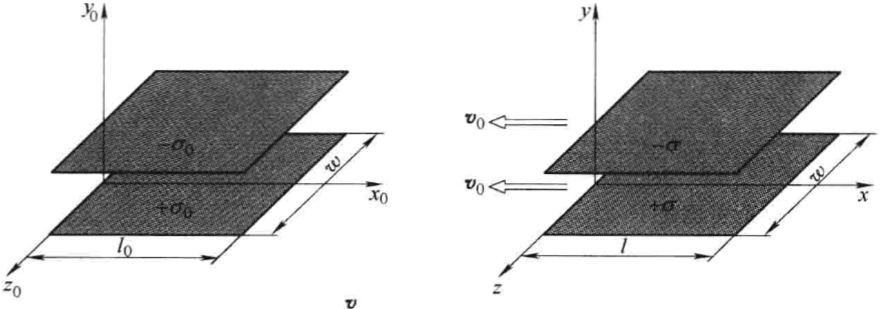
\includegraphics[width=\textwidth]{5-6.png}
    \caption{垂直运动方向电场}
  \end{minipage}
  \hfill
  % 第二张图片
  \begin{minipage}[t]{0.25\textwidth}
    \centering
    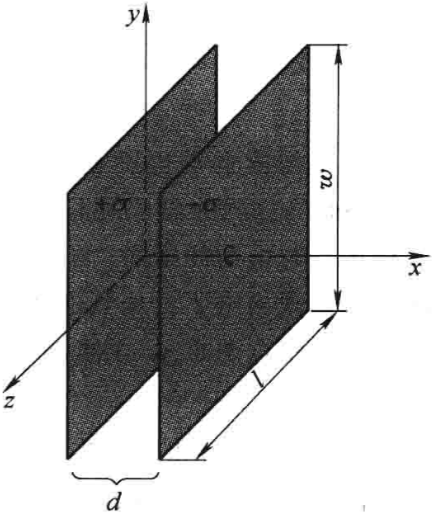
\includegraphics[width=\textwidth]{5-7.png}
    \caption{平行运动方向电场}
  \end{minipage}
\end{figure}

现在我们考察电容器在以$\v_0$的速度向右运动的参考系中的情况。在该参考系中电容器板向左运动,但电场仍然取下面的形式:
\[
E = \frac{\sigma}{\v_0}\hat{y}
\]

唯一的不同是电荷面密度。这是因为对称性告诉我们即便是电场发生了倾斜,板间电场叠加后仍然垂直于板面。

现在每个板上的总电荷保持不变,宽度不变,但是长度因为收缩效应而变小,于是单位面积电荷增加了因子:
\[
\gamma_0 = \frac{1}{\sqrt{1-\frac{v^2}{c^2}}},\quad \sigma = \gamma_0\sigma_0
\]
于是:
\[
E^{\perp} = \gamma_0E_0^{\perp}
\]
上标说明这个规则只对垂直$S$系运动方向的分量起作用。为了得到平行方向分量的情况,考虑右图,在这种情况下发生收缩的是板间距,然而电场不依赖于板间距$d$,于是
\[
E^{\parallel} = E_0^{\parallel}
\]

\begin{example}
  一个电荷量为$q$的点电荷静止于参考系$S_0$中的坐标原点,求其在以速度$v_0$相对$S_0$系向右运动的$S$系中的电场如何?

  \insertfig{5-8.png}{匀速运动点电荷的电场}{0.35}

在$S_0$系中,电场为:
\begin{align*}
E_{x0} &= \frac{1}{4\pi\varepsilon_0} \frac{q x_0}{(x_0^2 + y_0^2 + z_0^2)^{3/2}}, \\[6pt]
E_{y0} &= \frac{1}{4\pi\varepsilon_0} \frac{q y_0}{(x_0^2 + y_0^2 + z_0^2)^{3/2}}, \\[6pt]
E_{z0} &= \frac{1}{4\pi\varepsilon_0} \frac{q z_0}{(x_0^2 + y_0^2 + z_0^2)^{3/2}}.
\end{align*}

由上面的变换规则,我们有
\begin{align*}
E_x &= E_{x0} = \frac{1}{4\pi\varepsilon_0} \frac{q x_0}{(x_0^2 + y_0^2 + z_0^2)^{3/2}}, \\[6pt]
E_y &= \gamma_0 E_{y0} = \frac{1}{4\pi\varepsilon_0} \frac{q \gamma_0 y_0}{(x_0^2 + y_0^2 + z_0^2)^{3/2}}, \\[6pt]
E_z &= \gamma_0 E_{z0} = \frac{1}{4\pi\varepsilon_0} \frac{q \gamma_0 z_0}{(x_0^2 + y_0^2 + z_0^2)^{3/2}}.
\end{align*}

式中,场点 \( P \) 是用 \( S_0 \) 系中的坐标 \((x_0, y_0, z_0)\) 表示的,
用 \( S \) 系中的 \( P \) 点坐标表示更好。
由洛伦兹变换:
\begin{align*}
x_0 &= \gamma_0 (x + v_0 t) = \gamma_0 R_x, \\[4pt]
y_0 &= y = R_y, \\[4pt]
z_0 &= z = R_z.
\end{align*}

式中,\( \mathbf R \) 是从电荷 \( q \) 到 \( P \) 的矢量。

故
\begin{align*}
\mb{E} &= \frac{1}{4\pi\varepsilon_0} 
     \frac{q \gamma_0 \mathbf R}
          {(\gamma_0^2 R_x^2 + R_y^2 + R_z^2)^{3/2}} \\[6pt]
  &= \frac{1}{4\pi\varepsilon_0}
     \frac{q (1 - v_0^2/c^2) \mathbf R}
          {\bigl[R^2 (1 - (v_0^2/c^2)\sin^2\theta)\bigr]^{3/2}}. 
\end{align*}

\end{example}

前面讨论的还不是变换规则最一般的形式,因为我们是由电荷静止的$S_0$系开始推到的,在这个参考系中没有磁场。我们需考虑电场磁场均存在的某个参考系。我们考虑$S$系。对于电场:
\[
E_y = \frac{\sigma}{\v_0}
\]

注意到表面电流的形式为
\[
\mathbf K = \mp \sigma v_0 \hat x 
\]

对于这样的表面电流,我们先分析一个这样的表面产生的磁场。根据安培环路定理,我们对称地取图示的环路,得到:

\insertfig{5-9.png}{无限大电流平面产生磁场}{0.5}
\[
2Bl = \mu_0Kl \Rightarrow\mathbf B(z>0)=-\dfrac{\mu_0 K}{2}\,\hat y,\quad \mathbf B(z<0)=+\dfrac{\mu_0 K}{2}\,\hat y
\]

对于本题,两个磁场叠加,得到
\[
B_z = -\mu_0 \sigma v_0 
\]

在第三个参考系 $\overline{S}$ 中——该参考系相对 $S_0$ 向右以速度 $v$ 运动,场是
\begin{align*}
\overline{\mathbf E}_y &= \frac{\overline{\sigma}}{\varepsilon_0}, \qquad 
\overline{\mathbf B}_z = -\mu_0 \overline{\sigma} v 
\end{align*}

式中,$\overline v$ 是 $S$ 相对于 $S_0$ 的速度:
\begin{align*}
\overline v &= \frac{v + v_0}{1 + v v_0 / c^2}, 
\qquad 
\overline{\gamma} = \frac{1}{\sqrt{1 - \overline v^2 / c^2}} 
\end{align*}

而
\begin{align*}
\overline \sigma = \overline \gamma \sigma_0 
\end{align*}

剩下的只是用 $\mathbf E$ 和 $\mathbf B$表示
$\overline{\mathbf E}$ 和 $\overline{\mathbf B}$:
\begin{align*}
\overline E_y &= \left(\frac{\overline{\gamma}}{\gamma_0}\right)\frac{\sigma}{\varepsilon_0}, 
\qquad 
\overline B_z = -\left(\frac{\overline{\gamma}}{\gamma_0}\right)\mu_0 \sigma v 
\end{align*}

通过简单的代数运算,得到
\begin{align*}
\frac{\overline{\gamma}}{\gamma_0} 
&= \frac{\sqrt{1 - v_0^2 / c^2}}{\sqrt{1 - \overline v^2 / c^2}}
   = \frac{1 + v v_0 / c^2}{\sqrt{1 - v^2 / c^2}} 
   = \gamma \left( 1 + \frac{v v_0}{c^2} \right) 
\end{align*}

式中,与通常一样
\begin{align*}
\gamma = \frac{1}{\sqrt{1 - v^2 / c^2}} 
\end{align*}

于是我们代入得到:
\[
\overline{E_y} = \gamma(E_y-vB_z)
\]
\[
\overline{B_z} = \gamma(B_z-\frac{v}{c^2}E_y)
\]
这里利用了:
\[
c^2 = \frac{1}{\mu_0\v_0}
\]

同样的方法,只需要将平行板电容器由平行$xz$平面改为平行$xy$平面就可以得到剩下两个垂直分量的变换公式:
\[
\overline{E_z} = \gamma(E_z+vB_y)
\]
\[
\overline{B_z} = \gamma(B_y+\frac{v}{c^2}E_z)
\]
对于$x$分量我们已经证明了电场强度的$x$分量是不变的。下面我们利用螺线管考察磁场的$x$分量.
\insertfig{5-10.png}{由螺线管考察磁场}{0.5}

在$S$系中螺线管静止,螺线管内的磁场是:
\[
B_x = \mu_0 nI
\]
在$\overline{S}$系中,因为收缩效应单位长度上的匝数增加:
\[
\overline{n} = \gamma n
\]
另一方面,时间的延缓效应导致$\d \tau$时间内通过的电荷现在在$\d t$时间内通过,于是电流将会减小:
\[
\overline{I} = \frac{1}{\gamma}I
\]
于是得到:
\[
\overline{B_x} = B_x
\]

现在我们可以得到最终的变换公式了:
\begin{align*}
E_x &= E'_x,\\[4pt]
E_y &= \gamma\bigl(E'_y + v B'_z\bigr),\\[4pt]
E_z &= \gamma\bigl(E'_z - v B'_y\bigr),
\end{align*}
\begin{align*}
B_x &= B'_x,\\[4pt]
B_y &= \gamma\Bigl(B'_y - \frac{v}{c^2}E'_z\Bigr),\\[4pt]
B_z &= \gamma\Bigl(B'_z + \frac{v}{c^2}E'_y\Bigr).
\end{align*}

特殊情况:

(1)$S$系中无磁场,则:
\[
\overline{B} = -\frac{1}{c^2}(\mb{v}\times \overline{\mb{E}})
\]

(2)$S$系中无电场,则:
\[
\overline{E} = \mb{v}\times\overline{\mb{B}}
\]

\begin{example}
  求匀速运动的点电荷的磁场.

  注意到电荷静止参考系中没有磁场,于是:
  \[
  \mb{B} = -\frac{1}{c^2}(\mb{v}\times \overline{\mb{E}}) = -\frac{\mu_0}{4\pi}\frac{qv(1-v^2/c^2)\sin\theta}{[1-(v^2/c^2)\sin^2\theta]^{3/2}} \frac{\hat{\Phi}}{R^2}
  \]

  低速情况下,上式可以简化成:
  \[
  \mb{B} = \frac{\mu_0}{4\pi}\frac{q\mb{v}\times\mb{R}}{R^3}
  \]

  由此我们也可以大致看出,在一个运动电荷对另一个静止电荷作用的过程中,磁力与电力的比值大约是$\frac{v^2}{c^2}$量级。低速情况下磁力远小于电力。
\end{example}
\bibliographystyle{plainnat}
\begin{thebibliography}{99}
\bibitem{dawu} 胡其图, 李晟, 刘世勇, \textit{大学物理教程(AR版)}, 人民邮电出版社, 2023.
\bibitem{griffiths} D. J. Griffiths, \textit{Introduction to Electrodynamics}, Pearson, 2023.
\bibitem{zhaokaihua} 赵凯华, 陈熙谋, \textit{新概念物理教程:电磁学}, 高等教育出版社, 2006.
\bibitem{chengjiafu} 程稼夫, \textit{中学奥林匹克竞赛物理教程:电磁学篇}, 中国科学技术大学出版社, 2014.
\bibitem{huyouqiu} 胡友秋, 程福臻, 叶邦角, 刘之景, \textit{电磁学与电动力学(上册)}, 科学出版社, 2014.
\bibitem{chenbingqian} 陈秉乾, 舒幼生, 胡望雨, \textit{电磁学专题研究}, 北京大学出版社, 2001.

\end{thebibliography}

\end{document}
